\documentclass[10pt, headsepline,DIV14,BCOR0.5cm]{scrreprt}
\usepackage[utf8x]{inputenc}
\usepackage[T1]{fontenc}
\usepackage{arev}
\usepackage{booktabs}
\usepackage{parskip}
\usepackage{setspace} 
\usepackage{multicol}
\usepackage{natbib}
\usepackage{hyperref}
\usepackage{graphicx}
\usepackage{xcolor}
\usepackage{listings}
\usepackage{mdwlist}

\setlength{\parindent}{0cm}
\setlength{\parskip}{2em}
%\linespread{1.3}

\definecolor{lgrey}{gray}{0.98}
\definecolor{dgrey}{gray}{0.6}
\hypersetup{pdfborder=0 0 0, colorlinks=true, linkcolor=black, anchorcolor=black, citecolor=black, urlcolor=blue}
\widowpenalty=10000
\clubpenalty=10000


%% Set up code listings
\lstset{ %
basicstyle=\footnotesize,
numbers=left, 
numberstyle=\tiny,
breaklines=true, 
frame=single,
showspaces=false,               % show spaces adding particular underscores
showstringspaces=false,         % underline spaces within strings
showtabs=false,                 % show tabs within strings adding particular underscores
backgroundcolor=\color{lgrey},  % choose the background color. You must add \usepackage{color}
}

%% Define colours
\definecolor{lgrey}{gray}{0.98}
\definecolor{dgrey}{gray}{0.6}
\definecolor{dgreen}{RGB}{0,60,0}
\definecolor{greygreen}{RGB}{237,243,237}

% Title Page
\title{TRiCYCLE Users Manual}
\author{Peter Brewer, Daniel Murphy and Esther Jansma}
\publishers{\footnotesize{Cornell University, Ithaca, New York \\ Cultural Heritage Agency (RCE/OCW), Amersfoort, The Netherlands }}
\date{Version 0.2.3}

\renewcommand{\bibname}{References}


\begin{document}
\maketitle
\pagenumbering{roman}
\setcounter{page}{1}

\tableofcontents


\chapter{Acknowledgements}
\pagenumbering{arabic}
\setcounter{page}{1}

Funding for the development of TRiCYCLE has been provided by NWO section Humanities through the
DCCD project and through the various patrons of the Malcolm and Carolyn Wiener Laboratory for Aegean
and Near Eastern Dendrochronology.

We would like to thank the numerous contributors to the open source libraries used by TRiCYCLE and
its associated libraries. We would also like to thank Roland Aniol, Rémi Brageu, Pascale Fraiture,
Henri Grissino-Mayer, Patrick Hoffsummer, Bernhard Knibbe, George Lambert, Lars-Åke Larsson Catherine Lavier, Hubert
Leuschner, Martin Munro, Ian Tyers and Ronald Visser for assistance understanding many of the data
formats implemented.

\chapter{What is TRiCYCLE?}

TRiCYCLE is a universal dendrochronology file format converter. It currently has support for reading and
writing 22 different file formats:

\begin{table*}[htbp]
\label{tbl:supportedFormats}
\caption{Formats supported by TRiCYCLE}
\begin{center}
\begin{tabular*}{10cm}{ l @{\extracolsep{\fill}} c  c }
  \toprule
 Format & Read support & Write support\\
 \midrule

Belfast Apple      	 	& \checkmark  & \checkmark \\
Belfast Archive   	 	& \checkmark  &            \\
Besan\c{c}on		 	& \checkmark  & \checkmark \\
CATRAS			   	& \checkmark  & \checkmark \\
Comma Separated Values		& \checkmark  & \checkmark \\
Corina Legacy		   	& \checkmark  & \checkmark \\
DendroDB		   	& \checkmark  &            \\
Heidelberg		   	& \checkmark  & \checkmark \\
Microsoft Excel 97/XP/2000 	& \checkmark  & \checkmark \\
Microsoft Excel 2007 		& \checkmark  & \checkmark \\
Nottingham		 	& \checkmark  & \checkmark \\
ODF Spreadsheet		 	& \checkmark  & \checkmark \\
Oxford			 	& \checkmark  & \checkmark \\
PAST4			 	& \checkmark  & \checkmark \\
Sheffield		 	& \checkmark  & \checkmark \\
Topham			 	& \checkmark  & \checkmark \\
TRiDaS			 	& \checkmark  & \checkmark \\
TRIMS			 	& \checkmark  & \checkmark \\
Tucson			 	& \checkmark  & \checkmark \\
Tucson Compact		 	& \checkmark  & \checkmark \\
VFormat			 	& \checkmark  & \checkmark \\
WinDENDRO		 	& \checkmark  &            \\

\bottomrule
\end{tabular*}
\end{center}
\end{table*}


TRiCYCLE extracts both data and any metadata present in files and converts them to the Tree-Ring Data
Standard (TRiDaS) data model. As TRiDaS is capable of representing the full range of dendro data and
metadata, it is then possible to write out the file to any one of the supported formats.
Key features of TRiCYCLE are:

\begin{itemize*}
 \item Seamless support for units where possible
 \item Interpretation of all metadata
 \item Handling of different character sets and line feeds from different operating systems
 \item Comprehensive warning and exception system which provides detailed feedback when errors are
detected in files
\end{itemize*}


For a complete discussion of TRiCYCLE and its underlying libraries please see \citep{tricycle}.


\chapter{Installation}

TRiCYCLE is a Java application and so can be installed on any modern operating system. To make
installation more familiar though we have packaged it up into native installers for Windows, Mac OSX
and Linux. Download the relevant package for your operating system from the SourceForge \url{http://
tridas.sf.net} website.

\begin{description}
 \item[Windows] - Run the setup program and follow the steps. The program will be installed to your hard disk
and shortcuts added to your start menu. If you do not have Java installed on your system or
you do not have the required version the installer will provide you with assistance to do so.
 \item[Mac OSX] - Open the .dmg file in Finder. Drag the TRiCYCLE.app file into your Applications folder, or
wherever you'd like it installed. MacOSX comes pre-installed with Java so there is no need
to install it separately.
 \item[Linux] - An Ubuntu deb package is provided for TRiCYCLE. Install this package with your standard
package manager (e.g. sudo dpkg --install TRiCYCLE\_X.X.deb). It includes information
on the required dependencies therefore it should install everything you need if you are
running Ubuntu. On other distributions you may find that the dependencies do not install
automatically and the TRiCYCLE installation fails. If this is the case you will have to install
sun-java6-jre first manually.
\end{description}


\chapter{How to use TRiCYCLE}

The first step is to specify the format of your input file(s). Choose your input file format from the pull
down list on the File List page.  If you are uncertain what format your file is in, you can use Identify file format option in the help menu. Due to the fact that some formats are very similar, Corina may suggest the file is one of several formats.  If this is the case you will need to either check the file format descriptions in the appendices, or try each format in turn.

The next stage is to specify the file(s) that you would like to convert. This
can be done in a variety of ways:

\begin{itemize*}
 \item Click the browse button
 \item Use the \verb|File > Open| menu
 \item Drag files onto the dialog box from your file manager (e.g. Finder on MacOSX, My Computer on
Windows or Nautilus, Dolphin, Konqueror etc on Linux).
\end{itemize*}

Once you have your list of files prepared you can then go to the Convert tab.

On the Convert page, the next thing you need to do is select the desired output format from the drop down
list. Next, press the convert button and after a short delay your files should appear in the list below. At the
bottom of the window, you'll see a summary showing how many files were processed, how many of the
conversions failed and how many were converted successfully but with warnings.


The results of the conversion are shown in a tree view on the convert tab. Files that failed to convert are
highlighted by a red cross along with a message explaining what went wrong. Each file that converted
successfully and with no warnings is shown with a green tick icon below which are shown the output file
or files. Depending on the input and output formats chosen, a input file may be converted into one or more
output files as some formats can store just one series while others can store multiple series.


\begin{figure}
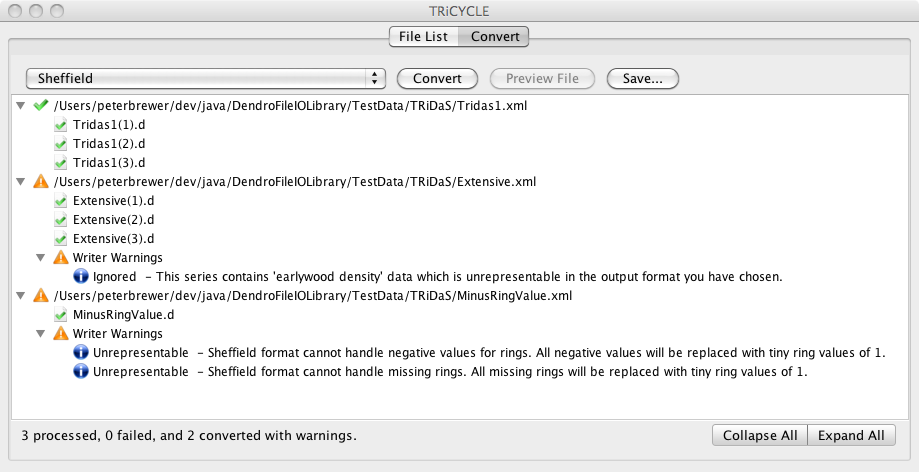
\includegraphics[width=\textwidth]{screenshot1.png}
\caption{Screen shot showing the conversion of three TRiDaS files into Sheffield
format. The second and third files both include warnings that the Sheffield format
is unable to fully represent all the data in the input files.} 
\label{fig:screenshot}
\end{figure}

If there were warnings produced during the conversion process, then the file will be marked with a orange
exclamation icon. Warnings can be associated with either the process of reading the input file, or writing
the output file. They can also be related to a single series within the file or the input file as a whole. The
warning messages are displayed to illustrate the context of the warning. Longer warnings will scroll of the
edge of the window, but if you hover your mouse over the warning a tool-tip will show the entire message.

If you would like to preview the result of the conversion process you can double click on the output files
and they will be displayed in a text viewer. This option is not, however, available for binary formats such
as CATRAS and Excel.

Once you are happy with the results of the conversion you can save the files permanently to disk by pressing
the save button. It will offer you the option of specifying which folder to save the files to.


\chapter{Options}

The options panel is available from the file menu. It is split into two sections: Reader config and Writer
config.

\section{Character sets}

The character set can be set for both the file being read and the file being written. The character set is
the system for pairing computer character codes with the character glyphs that we read. The widely
used standard was originally ASCII, but this does not include diacritic characters, and characters specific
to certain languages. There have since been many character encodings proposed (e.g ISO 8859-1 for
Western Europe and ISO 8859-7 for Greece) as well as some that are specific to Windows and Mac
operating systems (e.g. Windows-1252 and MacRoman). The character set that is becoming most widely
used is Unicode UTF-8. This is capable of representing all 107,000+ distinct characters while remaining
backwards compatible with ASCII for the 128 characters that it is able to represent.

If an incorrect character encoding is used to interpret a file, normally the majority of characters will display
correctly (where the character sets share the same encodings) but more unusual characters will be displayed
incorrectly - typically square boxes or question marks.

TRiCYCLE can using the NIO package to attempt to automatically detect which encoding a file is in.
Unfortunately, there is no full-proof way to do this, so by default, this feature is turned off. If you are
having problems with character encodings you may like to choose 'Automatic' in the charset box if you
have no idea what character encoding your file is in.

The character encoding is set to the default for the operating system you are running. For instance on
MacOSX this will be MacRoman and for Windows it will be Windows-1250. If you know your input file
is in a different encoding you should set it in the input charset box. If your output file needs to be read
on an operating system other than the one you are currently running, then you may like to override the
writer charset. Please note that for certain writers, the character set used is part of the file specification
(e.g. TRiDaS must be UTF-8). In this case your choice will be ignored.

The final complication with regards character sets is the line feed character(s). For historical reasons
different operating systems use different characters to represent a new line. Depending on the software
that is used to read a file, this can cause problems. TRiCYCLE itself will automatically adapt to files with
any type of line feed characters so reading files in TRiCYCLE will never be a problem. When writing
out files, TRiCYCLE will use the default line feed for the operating system you are running, unless you
choose a platform specific character set. For instance if you run TRiCYCLE on Windows and choose a
MacRoman writing charset, TRiCYCLE will use Mac style line feeds.


\section{Metadata editor}

TRiCYCLE works by reading in a data file and translating it into the TRiDaS data model. TRiDaS has
a rich array of fields to represent all manner of dendro data and metadata. Although most of these are
optional, the TRiDaS specification requires that a handful of these are always filled in. Unfortunately many
of the legacy data formats do not contain information for these mandatory fields, therefore TRiCYCLE
must fill these with default values. You will most commonly see these defaults as 'Unnamed object' etc in
your output file. The metadata editor enables you to override these default values.

Clicking on the reader metadata editor button in the options window will give a table of all the metadata
fields that will be set automatically by TRiCYCLE along with their current values. You can change most
of these with the exception of those that are required to be a controlled vocabulary. These will require a 
more complicated interface which we haven't had time to implement yet. The third column in the editor is
a tick box to specify whether the value is overriding or not. If ticked, the value specified in this editor will
be used regardless of whether a value can be extracted by TRiCYCLE from the input data files.

An identical editor is available for the writer. These are the default values used by the writer code for
your chosen output format. For instance, TRiDaS does not require that a start year field be set (as in the
case of relatively dated series), whereas some output formats do require such a field. If an input file does
not contain start year information then some writers need to know which default value for start year to
use. Like for the input metadata editor, you can set fields to `overriding' which means they will be used
regardless of whether this information is available in the input dataset.

\section{Naming convention}

Some file formats can contain just one data series while others can contain many. When converting from
a multi-series format to a single series format this means that one input file is converted to multiple output
files. The naming convention is used to determine how to name the output files. The naming convention
relates to the filename itself and not the file extension. The file extension is specific to the output format
chosen (e.g. Heidelberg files are .fh and TRiDaS files are .xml).

\begin{description}
 \item[Numerical] - This is the default naming convention. It uses the name of the input data file and
appends an incrementing number if more than one output file is produced.
 \item[UUID] - This gives all output files a random named based on Universally Unique Identifiers
(UUIDs). This is a 36 character hexadecimal code which due to the astronomically
large number of possible combinations is guaranteed to be universally unique. A
typical filename will look like: 550e8400-e29b-41d4-a716-446655440000.
 \item[Hierarchical] - This uses the hierarchical structure of the TRiDaS data model to provide a meaningful
name for the output file. It joins together the title of each entity in the file beginning
with the project name through to the series name. For files that contain multiple series,
the name will contain details of all the entities shared by all the series in the file. For
example, if a file contains several series from the same sample, then the file name
will be projectTitle-objectTitle-elementTitle-sampleTitle. If the file contains several
series from different samples of the same object, then the file would be projectTitle-
objectTitle. If multiple output files end up with the same name then like the numerical
convention described above, the files will have an incremental number appended to
the end. Unfortunately, most input data files do not contain rich name information
so files end up being called unnamedProject-unnamedObject-unnamedElement etc.
This convention is therefore more appropriate when converting from TRiDaS to other
formats.
 \end{description}

\section{Privacy options}

On first launch, TRiCYCLE will ask permission to collect anonymous usage data.  This information will help us focus future development efforts, but if you prefer not to submit this data, you can decline.  You can change your mind at any time by checking or unchecking the tick box in the options dialog.

By default TRiCYCLE also periodically checks for the availability of updates on the tridas.org website.  If you would prefer to check manually you can turn this features and either use the `Check for updates' entry in the Help menu, or visit the TRiDaS website with your normal web browser.

\chapter{Help and more information}

The best place to start is through the TRiDaS website (\url{http://www.tridas.org}) and the
Dendro Data Standards forum. The forum is a email list for the discussion of TRiDaS and other dendro
data standards issues. It is open for all to join by emailing Peter Brewer (\href{mailto:p.brewer@cornell.edu}{p.brewer@cornell.edu}).

TRiCYCLE is an open source product therefore we are very pleased to welcome anyone that would
like to assist in its development. This obviously includes programmers, but also people willing to help
with documentation and translations too. To find out more information please contact Peter Brewer
(\href{mailto:p.brewer@cornell.edu}{p.brewer@cornell.edu}).


\bibliographystyle{elsarticle-harv}
\bibliography{DendroTech}
\addcontentsline{toc}{chapter}{\hspace{5.5mm}References}


\part*{Appendix - File format descriptions}

\appendix

\chapter{Belfast Apple}
\label{txt:fileFormatsStart}
\index{File formats|(}

\index{File formats!Belfast Apple|(}
\begin{table*}[htbp]
\label{summary:belfastApple}
\begin{center}
\begin{tabular*}{15cm}{ l @{\extracolsep{\fill}} p{9cm} }
  \toprule

Format name     	 & Belfast Apple \\
Other name(s)      	 & None known \\
Type      	 	 & Text file \\
Extension(s)      	 & Various (typically txt and dat) \\
Read/write support     	 & Read and write \\
Reference implementation & No original software is known to exist so TRiCYCLE is proposed as the reference implementation \\
Data / metadata      	 & Data only with comment \\
Calendar type		 & n/a \\
Absolute dating support	 & No \\
Undated series support   & Yes \\
Relative dating support  & No \\
Multi series support	 & No \\
Original designer	 & John Pilcher \\

\bottomrule
\end{tabular*}
\end{center}
\end{table*}


\section{Description}
Belfast Apple is a simple text file format (see also \hyperref[summary:belfastArchive]{Belfast Archive})
originating from the Queens University Belfast lab and originally designed for use on an Apple II computer.
This format is not known to be actively used but a large amount of data (especially at Belfast) is archived
in this format.

\begin{itemize*}
 \item Line 1 - name of the site or object the data refers to.
 \item Line 2 - identifier for the sample the data refers to.
 \item Line 3 - number of data values in the file
 \item Lines 4+ - line feed delimited data values as integers in 1/100th mm
 \item Final line contains a comment typically starting with `COMMENT -'
\end{itemize*}

\newpage
\section{Example file}

\begin{lstlisting}
EXAMPLE SITE
A1805
106
188
165
184
112
103
111
239
226
132
143
146
140
100
176
139
124
115
78
80
156
75
110
80
130
83
157
99
115
102
110
108
87
135
107
96
70
128
119
86
101
106
129
88
101
151
106
97
110
97
91
93
100
124
99
134
125
105
96
107
142
100
COMMENT -   PB 15-NOV-99

\end{lstlisting}
\index{File formats!Belfast Apple|)}



\chapter{Belfast Archive}
\index{File formats!Belfast Archive|(}

\begin{table*}[htbp]
\label{summary:belfastArchive}
\begin{center}
\begin{tabular*}{15cm}{ l @{\extracolsep{\fill}} p{9cm} }
  \toprule

Format name     	 & Belfast Archive\\
Other name(s)      	 & None known\\
Type      	 	 & Text file\\
Extension(s)      	 & Various (typically arx, txt and dat)\\
Read/write support     	 & Read only\\
Reference implementation & No original software is known to exist so TRiCYCLE is proposed as the reference implementation\\
Data / metadata      	 & Data with limited metadata\\
Calendar type		 & Gregorian\\
Absolute dating support	 & Yes \\
Undated series support   & No \\
Relative dating support  & No \\
Multi series support	 & Yes \\
Original designer	 & Martin Munro\\

\bottomrule
\end{tabular*}
\end{center}
\end{table*}

\section{Description}

Belfast Archive is a simple text file format based on the original \hyperref[summary:belfastApple]{Belfast Apple} format at the Queens University Belfast lab. It shares the same features as Belfast Apple but with the addition of a number of metadata fields at the end of the file.

\begin{itemize*}
 \item Line 1 - name of the site or object the data refers to.
 \item Line 2 - identifier for the sample the data refers to.
 \item Line 3 - number of data values in the file
 \item Lines 4+ - line feed delimited data values as integers in 1/100th mm
 \item The lines \verb|"[[ARCHIVE]]"| and \verb|"[[ END OF TEXT ]]"| denote the start and finish of the metadata section  
\end{itemize*}

The metadata section contains the following lines:

\begin{itemize*}
    \item  Line 1 - start year as an integer.
    \item  Line 2 - unknown
    \item  Line 3 - Double representing the resolution of data values e.g. .1= 1/10ths mm, .01 = 1/100th mm, .001 = microns etc
    \item  Line 4 - unknown
    \item  Line 5 - unknown
    \item  Line 6 - unknown
    \item  Line 7 - title of the data series
    \item  Line 8 - unknown
    \item  Line 9 - unknown 
\end{itemize*}

\section{Example file}

\begin{lstlisting}
EXAMPLE SITE
1
176
342
338
334
409
362
308
360
264
325
318
51
48
47
60
49
48
"[[ARCHIVE]]"
1277
9177
.01
1.035795
0.212144
BOB 25/03/95
EXAMPLE SITE #01
Pith F Sap 32
""
"[[ END OF TEXT ]]"
\end{lstlisting}
\index{File formats!Belfast Archive|)}


\chapter{Besan\c{c}on}
\index{File formats!Besan\c{c}on|(}
\index{File formats!SYLPHE|see{Besan\c{c}on}}
\begin{table*}[htbp]
\label{summary:besancon}
\begin{center}
\begin{tabular*}{15cm}{ l @{\extracolsep{\fill}} p{9cm} }
  \toprule

Format name     	 & Besan\c{c}on \\
Other name(s)      	 & SYLPHE\\
Type      	 	 & Text file\\
Extension(s)      	 & txt\\
Read/write support     	 & Read and write\\
Reference implementation & \\
Data / metadata      	 & Data and some structured metadata\\
Calendar type		 & Gregorian\\
Absolute dating support	 & Yes\\
Undated series support   & Yes\\
Relative dating support  & No \\
Multi series support	 & Yes \\
Original designer	 & Georges Lambert\\

\bottomrule
\end{tabular*}
\end{center}
\end{table*}

\section{Description}

The Besan\c{c}on format is most commonly used in a number of French laboratories. The format allows for multiple series in the same file. Each series (or element block in Lambert's notation) is made up of a header line, optional metadata and a data block each of which are delimited by a line feed. 


The header line begins with a dot character, then one or more spaces, then an element name (without spaces) followed by a space and any number of ignored characters.

The metadata fields are space or line feed delimited. Each field is recorded using a key of three letters. The format allows for the full spelling out of the field if preferred, but it is the first three letters that are read by software so LON is the same as LONGEUR. Some fields are `unimodal' in that their presence is all that is required e.g. CAM means that cambium was observed. Other fields are `bimodal' which means they require a value to be associated with them. In this case the field key is followed by a space and then an integer or string value e.g. POS 1950. The accepted metadata fields are as follows:
    \begin{description}
          \item[LON] Number of data values
          \item[POS] The temporary first ring date given relatively to a group
          \item[ORI] The year for the first ring
          \item[TER] The year for the last ring. Should be the same as ORI + LON
          \item[MOE] Pith present
          \item[CAM] Cambium present
          \item[AUB] Number of the first sapwood ring 
    \end{description}   
All other information in the metadata block should be ignored. This feature is often used to allow the inclusion of multi-line comments. 

The data block begins with the marker line VAL (like metadata keys, subsequent characters are ignored so sometimes the rest of this line is used for comments). Subsequent lines contain integer values delimited by a space or line feed. Missing rings are marked with a comma character and the end of the data is marked with a semicolon. 


\section{Additional information}

\begin{itemize*}
  \item There is nothing in the specification to say what precision the data values should be in. Following conversations with users it appears that Besan\c{c}on files are mostly 1/100th mm but this is not always the case. Some files include a Précision field, but this is not documented or standardised.
  \item There are a number of additional fields that are commonly used but which do not appear in the format specification. These are also supported by the DendroFileIOLib
  \begin{description}
    \item[ESP] Species
    \item[ECO] Bark present  
  \end{description}
\end{itemize*}

\section{Example file}
\begin{lstlisting}
 . abc22/43
 Lon 129
 Esp quercus sp  Nat lambris
 Precision 1/100
 Moelle non presente
 Aub 0   
valeurs
  149  119  156  146  170  187  197  146  191  177
  137  108  160  108  120  177  136  174  190  109
  189  176  170  162  114  126  133  152  146  127
  119  131  146  133  147   82   57   77   77   82
   96   49   97   76   88   82   72   83   81   90
   85   87   78  104  111  132  141  105  104  120
  111  121  115   89   94   88   90  115  111  106
  107  120   80   92   98   84   97   82  100   86
   99   65   85  113   90   82   57   57   99   94
   95  105  120  110   93   96  131  133  123  122
  113  119   95  127   88  104    ,    ,    ,    ,
    ,    ,    ,    ,    ,    ,    ,    ,    ; 
\end{lstlisting}
\index{File formats!Besan\c{c}on|)}


\chapter{CATRAS}
\index{File formats!CATRAS|(}
\begin{table*}[htbp]
\label{summary:catras}
\begin{center}
\begin{tabular*}{15cm}{ l @{\extracolsep{\fill}} p{9cm} }
  \toprule

Format name     	 & CATRAS\\
Other name(s)      	 & None known\\
Type      	 	 & Binary\\
Extension(s)      	 & cat\\
Read/write support     	 & Read only\\
Reference implementation & CATRAS\\
Data / metadata      	 & Data and some structured metadata\\
Calendar type		 & Gregorian\\
Absolute dating support	 & Yes\\
Undated series support   & Yes\\
Relative dating support  & No\\
Multi series support	 & No\\
Original designer	 & Roland Aniol \\

\bottomrule
\end{tabular*}
\end{center}
\end{table*}

\section{Background}
The CATRAS format \citep{catras} is the only known binary dendro data format. As such it can't be read by a simple text editor, and can't be imported by spreadsheet or database programs. The format was designed by Roland Aniol for use in his program of the same name. The binary nature of the format means the files are typically much smaller than text files containing similar data. The closed nature of the format originally meant that users were tied to the application.  The fact that users can't manually edit the file means that the validity of files is not a problem like it is with most other dendro formats.

The format was originally decoded in the early 1990's and permission was granted by Aniol for a converter to be included in Henri Grissino-Mayer's CONVERT5 application. Subsequently others have independently released application and code that can read CATRAS files to a greater or lesser extent. 

Following its original release in 1983, CATRAS was updated several times, the most recent version (v4.42) was released in 2010. The code in DendroFileIOLib is based on Matlab, Fortran and C code of Ronald Visser, Henri Grissino-Mayer and Ian Tyers. 

\section{Reading byte code}

Reading byte code is more complicated than reading text files. Each byte is 8-bits and therefore can represent up to 256 values. Depending on the type of information each byte contains, the bytes are interpreted in one of four ways: 

\subsection{Strings} Some of the bytes in CATRAS files contain character information. In this case each byte represents a letter. In java an array of bytes can be directly decoded into a string. 

\subsection{Integers} As a byte can only represent 256 values, whenever an integer is required it is stored as a byte pair. Each byte pair consists of a least significant byte (LSB) and a most significant byte (MSB). The order that they appear in files typically varies between platforms and is known as 'endianness'. As CATRAS solely runs on Microsoft (x86) processors we can safely assume that all CATRAS files will be using little-endian (i.e. LSB MSB). The counting in a byte pair therefore works as follows: 

\begin{table*}[htbp]
\begin{center}
\begin{tabular*}{5cm}{@{\extracolsep{\fill}} r r r }
  \toprule
Value & LSB & MSB\\
\midrule
0 & 0 & 0\\
1 & 1 & 0\\
\dots & \dots & \dots\\
255 & 255 & 0\\
256 & 0 & 1\\
257 & 1 & 1\\
258 & 2 & 1\\
\dots & \dots & \dots\\
\bottomrule
\end{tabular*}
\end{center}
\end{table*}

A byte pair can therefore store 256x256=65536 values (more than enough for most number fields). Matters are complicated though by the need to store negative numbers. Pairs with an MSB<=128 are positive, while pairs with an MSB ranging from 255 to 128 (counting backwards) represent negative values:

\begin{table*}[htbp]
\begin{center}
\begin{tabular*}{5cm}{@{\extracolsep{\fill}} r r r }
  \toprule
Value & LSB & MSB\\
\midrule
-1 & 255 & 255 \\
-2 & 254 & 255 \\
-3 & 253 & 255 \\
-4 & 252 & 255 \\
\dots & \dots & \dots\\
\bottomrule
\end{tabular*}
\end{center}
\end{table*}

\subsection{Real numbers}

Statistics like arithmetic mean, standard deviation, first-order autocorrelation, and mean sensitivity are given for both all the ring widths and the ring widths in an optional restricted part of the series. The real numbers are given in standard format defined by the IEEE 754 Standard for Floating-Point Arithmetic.

\subsection{Categories}

Categories are typically recorded as single bytes as most categories have just a few possible values. They can therefore be conceptualized as being integers where 0=first option, 1=second option etc. The exception to this is for species because there are more than 256 species. In this case, a byte pair is used in exactly the same way as described for integers above. The only problem for species is that the codes are unique to each laboratory and refer to values enumerated in a separate '.wnm' file. Without this dictionary the species code is of little use. 

\subsection{Dates}
The date of the creation of the series and the date of the last amendment to the series are stored as three single bytes each, one for day, one for month, and one for year. The year is stored with an offset of 1900. Therefore numbers from 1 to 100 belong to the 20th century (calendar year 1901 to 2000) and numbers from 101 to 200 belong to the 21th century (calendar year 2001 to 2100). 

\section{Metadata}

The first 128 bytes contain the file header information and the remainder of the file contains the ring-width data and sample depth data (if series is a chronology). If a series is only partly suitable for further analysis then this indicated in bytes 49--52. The quality code at position 58 is an overall rating for the series. This helps to exclude poor series from analyses other than dating. 

\begin{table}[htbp]
\begin{center}
\begin{tabular*}{\textwidth}{r c l p{8cm} }
  \toprule
Bytes & Data type & Field & Description \\
\midrule
1--32	& C & Series name & \\
33--40 & C &  Series code. Must be upper case and match file name.& \\
41--44 & C &File extension & \\
45--46 & I & Series length & \\
47--48 & I & Sapwood length &\\
49--50 & I & First valid ring & Used if a portion of the series is unreliable \\
51--52 & I & Last valid ring & Used if a portion of the series is unreliable \\
53       & B & Scope & 1=pith; 2=waldkante; 3=pith to waldkante; 4=bark; 5=pith to bark \\
54       & B & State of last ring & 0=last ring complete; 1=last ring only early wood \\
55--56 & I & First ring & Calendar year of first ring: 0=not dated; <0=B.C.; >0=A.D. \\
57       & B &  & Number of valid characters in series name\\
58       & B & Quality code& 0=not known; 1=very good \ldots 5=uncertain \\
59--60 & I & Species code & Requires an associated catras.wnm file \\
61--63 & D & Creation date & DMY, Y offset 1900 \\
64--66 & D & Last updated & DMY, Y offset 1900 \\
67       & B & Real number format & normally 1=IEEE \\
68       & B & Type of series & 0=ring widths; 1=early wood widths; 2=late wood widths\\
69--81 &  &  & Reserved \\
82       & C & Special sources & A=averaged; D=digitized; E=extern; H=manual input \\
83       & B & Protection & 0=no protection; 1=not to be deleted; 2=not to be amended \\
84       & B & File type & 0=raw; 1=tree curve; 2=chronology \\
85--88 & C & Creator & Initials of creator\\
\midrule
\multicolumn{4}{l}{\textit{Statistics for total series}} \\
89--92 & R & &Arithmetic mean  \\
93--95 & R & &Standard deviation  \\
96--100 & R & &First-order autocorrelation \\
101--104 & R & &Mean sensitivity  \\
105--106 & I & &Number of rings for mean  \\
107--108 & I & &Number of rings for autocorrelation  \\
\midrule
\multicolumn{4}{l}{\textit{Statistics for restricted part of series}} \\
109--112 & R & &Arithmetic mean  \\
113--116 & R & &Standard deviation  \\
117--120 & R & &First-order autocorrelation \\
121--124 & R & &Mean sensitivity  \\
125--126 & I & &Number of rings for mean  \\
127--128 & I & &Number of rings for autocorrelation  \\
\bottomrule
\end{tabular*}
\end{center}
\label{tbl:catrasMetadata}
\caption{Summary of the metadata portion of CATRAS files.  Data types are: strings (C); integers (I); real numbers (R); binary categories (B); and dates (D).  Bytes 89--128 contain descriptive statistics for the file, bytes 89--108 concerning the entire series, and bytes 109--128 a subset of the series where some poor quality data have been excluded.}
\end{table}


%\begin{itemize*}
%\item 1-32 - Series name
%\item  33-40 - Series code
%\item  41-44 - File extension
%\item  45-46 - Series length
%\item  47-48 - Sapwood length
%\item  49-50 - Start year
%\item  51-52 - End year
%\item  53 - 1=pith 2=waldkante 3=pith to waldkante
%\item  54 - 1 = ew only last ring
%\item  55-56 - Start year
%\item  59-60 species also needs a catras.wnm file
%\item  61-63 - Creation date
%\item  64-66 - Amended date
%\item  67 - Sapwood
%\item  68 - 1=valid stats
%\item  69-75 - dated?
%\item  84 - 0=raw 1=treecurve 2=chronology
%\item  85-86 - User id
%\item  89-92 - Average width
%\item  93-95 - Standard deviation
%\item  96-100 - Autocorrelation
%\item  101-104 - Sensitivity 
%\end{itemize*}


\section{Data}

The remaining bytes in the file contain the actual data values stored as integer byte pairs. All data are stored in multiples of 128 bytes. If the number of data bytes given in the header at position 45--46 is not a multiple of 128 the file is padded with extra bytes accordingly. Padded bytes should be ignored. 

\subsection{Ring widths}

Ring widths are stored in hundredths of a millimetre in the same order as the tree had been grown. When working with archaeological or geological wood it might occur that a particular ring is damaged and therefore its width cannot be determined precisely. To indicate that fact and to exclude this particular ring from further calculations its measured width is stored negative. In the CATRAS program a negative ring width will be taken into account neither in the calculation of tree curves and chronologies nor in the statistics or in comparisons with other series.

\subsection{Chronologies}

Chronology files are indicated at position 84 in the file header and contain additional data in respect to raw data files. After the block of ring width data three additional data blocks follow. Firstly the number of ring widths averaged at a particular position follows (the sample depth). Then the number of series with the same trend between subsequent ring widths at a particular position follows. Then the number of series with the opposite trend between subsequent ring widths at a particular position follows. All data blocks are stored in multiples of 128 bytes. If the number of data bytes given in the header at position 45-46 is not a multiple of 128 each block is padded with extra bytes accordingly. Padded bytes should be ignored. 



\index{File formats!CATRAS|)}

\chapter{Comma Separated Values}
\index{File formats!CSV|(}
\index{File formats!Comma Separated Values|see{CSV}}
\begin{table*}[htbp]
\label{summary:csv}
\begin{center}
\begin{tabular*}{15cm}{ l @{\extracolsep{\fill}} p{9cm} }
  \toprule

Format name     	 & Comma Separated Values\\
Other name(s)      	 & CSV \\
Type      	 	 & Text file\\
Extension(s)      	 & Various (typically txt or csv)\\
Read/write support     	 & Read and write \\
Reference implementation & n/a\\
Data / metadata      	 & Data only\\
Calendar type		 & Gregorian\\
Absolute dating support	 & Yes\\
Undated series support   & No\\
Relative dating support  & No\\
Multi series support	 & No\\
Original designer	 & n/a\\

\bottomrule
\end{tabular*}
\end{center}
\end{table*}

\section{Description}

Comma separated values format is a simple text format for representing tabular data. It is not specific to dendrochronology data and is supported by most spreadsheet and database applications. Data is delimited into columns using a comma character to indicate cell boundaries.

Support for CSV files in TRiCYCLE is limited to a particular layout of data.  The expected layout is the same as for Excel and ODF spreadsheet files:

\begin{itemize*}
 \item Row 1 - Header names for each column
 \item Column A - Year values
 \item Column B+ - One column for each series containing data values. Cells are left empty if no data is available for a series because it does not extend to a particular year. Data must be continuous for each series, so missing/unmeasured rings should be included as zero.
\end{itemize*}

\newpage
\section{Example file}

\begin{lstlisting}
Year,MySample1,MySample2
500,0.33,
501,0.26,0.26
502,0.2,0.2
503,0.14,0.14
504,0.08,0.08
505,0.02,0.02
506,0.2,0.2
507,0.14,0.14
508,0.08,0.08
509,0.2,
510,0.33,
511,0.08,
512,0.33,
513,0.22,
\end{lstlisting}
\index{File formats!CSV|)}

\chapter{Corina Legacy}
\index{File formats!Corina Legacy|(}

\begin{table*}[htbp]
\label{summary:corina}
\begin{center}
\begin{tabular*}{15cm}{ l @{\extracolsep{\fill}} p{9cm} }
  \toprule

Format name     	 & Corina Legacy\\
Other name(s)      	 & Corina\\
Type      	 	 & Text file\\
Extension(s)      	 & Various including raw, rec, ind, cln, sum)\\
Read/write support     	 & Read and write\\
Reference implementation & Corina\\
Data / metadata      	 & Data and some structured metadata\\
Calendar type		 & Gregorian\\
Absolute dating support	 & Yes\\
Undated series support   & No\\
Relative dating support  & Yes\\
Multi series support	 & No\\
Original designer	 & Robert `Mecki' Pohl\\

\bottomrule
\end{tabular*}
\end{center}
\end{table*}

\section{Description}

The Corina Legacy format is the file format used by the Corina software prior to version 2, when it transferred to using TRiDaS. The format was originally designed for use with the MS-DOS version of Corina but was also used as the native file format in the later Java versions (up to and including v1.1).

A Corina file contains yearly data (ring-width and number of samples for that year), some fixed metadata, and optionally weiserjahre data and a listing of element samples (for summed samples).

The title comes first, on a line by itself, followed by a blank line. The title is repeated later, so this is only to make it easier for people or external programs to read the title.

The \emph{metadata section} comes next. The syntax is \verb|;TAG| value. Tags are all uppercase. Their order is fixed. Some values are terminated by a newline, others by the next semicolon. Valid tags, and their internal names are: 

\begin{itemize*}
 \item ID - 8 character ID used when exporting to Tucson format
\item  NAME - Name of the series
\item  DATING - Either R (relative) or A (absolute)
\item  UNMEAS\_PRE - Number of unmeasured rings towards the pith
\item  UNMEAS\_POST - Number of unmeasured rings towards the bark
\item  FILENAME
\item  COMMENTS, COMMENTS2 etc - Free text comments
\item  TYPE - either C (core), H (charcoal) or S (section)
\item  SPECIES
\item  SAPWOOD - Count of sapwood rings
\item  PITH - either P (present), * (present but undateable), or N (absent)
\item  TERMINAL - either B (bark), W (waney edge), v (near edge), vv (unknown)
\item  CONTINUOUS - referring to the outer ring, either C (continuous), R (partially continuous) or N (not continuous)
\item  QUALITY - either + (one unmeasured ring), ++ (more than one unmeasured ring)
\item  FORMAT - either R (raw) or I (indexed)
\item  INDEX\_TYPE - type of index used
\item  RECONCILED - Y or N indicating whether the series has been reconciled against another series 
\end{itemize*}

The \emph{data section} comes next and this always starts with the line ;DATA and for reasons lost in time there are nine spaces afterwards.

Data lines come in pairs, the first line containing the year and data values, the second containing the sample depth/count for each value. For reasons unknown, the first and last data line pair have a slightly different syntax to the others. 

\begin{itemize*}
 \item First data line begins with a space and an integer for the first year in the line. There then follows 9 spaces followed by the integer data value for the first ring. The remaining data values (often less than a full decades worth) on that line follow as integers left padded by spaces to take up 6 characters.
\item  The sample depth line that pairs with this follows next starting with 16 spaces, followed by the sample depth value enclosed in square brackets. The remaining sample depth values follow in square brackets left padding with spaces to take up 6 characters.
\item  Next comes the first normal data line. This begins with a space, followed by an integer year value. The data values follow as integers left padded by spaces to take up 6 characters. A data line has a decades worth of data values.
\item  Next comes the normal sample depth line. It begins with 7 spaces followed by each of the sample depth values enclosed in square brackets and left padded with spaces up to 6 characters.
\item  Data lines continue in pairs until the last line is reached. This is the same as a normal data line except it includes an extra data value 9990 as a stop marker. This data line may have less than a full decade of values.
\item  The final sample depth line is the same as normal except it is shifted left by 4 characters. A sample depth value is also included for the dummy 9990 stop marker year. 
\end{itemize*}

Following the data block there is a blank line and two option blocks of data that are only included if the file is a chronology file.

The next block of information in a chronology file is denoted by a line ;ELEMENTS. The following lines contain the file names of the data files that have contributed to the creation of the chronology.

Following this is an optional block denoted by the line ;weiserjahre followed by the weiserjahre data. Each weiserjahre data line begins with a space followed by a integer year value for the first year in the line. The weiserjahre value is left padded with spaces to fill 6 characters and the value itself is written as X/Y where X is the number of samples that show an upward trend in width; and Y is the number of samples that show a downward trend in width. The weiserjahre value is forward facing so the value for ring 1001 shows the trend between ring 1001 and 1002. There is therefore one less weiserjahre value in the final row than there are ring-widths.

The final line of Corina data files contains the author's name preceded by a tilde. 

\newpage
\section{Example file}

\begin{lstlisting}
Trebenna, Byzantine Fortress, NW tower 1AB

;ID 907010;NAME Trebenna, Byzantine Fortress, NW tower 1AB;DATING R;UNMEAS_PRE 1;UNMEAS_POST 1
;FILENAME G:\DATA\TRB\TRB1AB.SUM


;TYPE S;SPECIES Juniperus sp.;FORMAT R;PITH +
;TERMINAL vv;CONTINUOUS N;QUALITY +
;RECONCILED Y
;DATA         
 1001         125   219   207   139    62   107    29    91    65
                [1]   [1]   [1]   [1]   [1]   [1]   [1]   [1]   [1]
 1010    71   132    74   150    75   156   122    81    46    57
          [1]   [1]   [1]   [1]   [1]   [1]   [1]   [1]   [1]   [1]
 1020   147    78    89   126    73   121    67    71    64   129
          [1]   [1]   [1]   [1]   [1]   [1]   [1]   [1]   [1]   [1]
 1030   149   155   122   126    53   136    90    65   100    67
          [1]   [1]   [1]   [1]   [1]   [1]   [1]   [1]   [1]   [2]
 1040    67   101   132   102    40    67    42    36    62    29
          [2]   [2]   [2]   [2]   [2]   [2]   [2]   [2]   [2]   [2]
 1050    30    44    46    40    34    61    55    29    44    63
          [2]   [2]   [2]   [2]   [2]   [2]   [2]   [2]   [2]   [2]
 1060    62    38    22    26    26    28    37    21    21    27
          [2]   [2]   [2]   [2]   [2]   [2]   [2]   [2]   [2]   [2]
 1070    17    18    50    21    33    12    17    16    27    20
          [2]   [2]   [2]   [2]   [2]   [2]   [2]   [2]   [1]   [1]
 1080    18    11     9     8  9990
      [1]   [1]   [1]   [1]   [1]

;ELEMENTS 
G:\DATA\TRB\TRB1A.REC
G:\DATA\TRB\TRB1B.REC
;weiserjahre   
 1001   1/0      0/1      0/1      0/1      1/0      0/1      1/0      0/1      1/0   
 1010   1/0      0/1      1/0      0/1      1/0      0/1      0/1      0/1      1/0      1/0   
 1020   0/1      1/0      1/0      0/1      1/0      0/1      1/0      0/1      1/0      1/0   
 1030   1/0      0/1      1/0      0/1      1/0      0/1      0/1      1/0      0/1      1/1   
 1040   2/0      2/0      0/2      0/2      2/0      0/2      0/2      2/0      0/2      2/0   
 1050   2/0      1/1      0/2      0/2      2/0      0/2      0/2      2/0      2/0      1/1   
 1060   0/2      0/2      2/0      1/1      2/0      2/0      0/2      1/1      2/0      0/2   
 1070   1/1      2/0      0/2      2/0      0/2      2/0      1/1      1/0      0/1      0/1   
 1080   0/1      0/1      0/1   
~ Unknown User
\end{lstlisting}
\index{File formats!Corina Legacy|)}




\chapter{DendroDB}
\index{File formats!DendroDB|(}

\begin{table*}[htbp]
\label{summary:dendrodb}
\begin{center}
\begin{tabular*}{15cm}{ l @{\extracolsep{\fill}} p{9cm} }
  \toprule

Format name     	 & DendroDB \\
Other name(s)      	 & \\
Type      	 	 & Text file\\
Extension(s)      	 & dat \\
Read/write support     	 & Read only\\
Reference implementation & DendroDB website\\
Data / metadata      	 & Data and some structured metadata\\
Calendar type		 & Astronomical\\
Absolute dating support	 & Yes\\
Undated series support   & No\\
Relative dating support  & No\\
Multi series support	 & Yes\\
Original designer	 & Simon Brewer\\

\bottomrule
\end{tabular*}
\end{center}
\end{table*}

\section{Description}

The DendroDB format is an export file format produced by the \href{http://dendrodb.cerege.fr/indexBAD.htm}{DendroDB website/database}. There is no known software that can natively read DendroDB files so a `writer' for this format has not been developed.

The format is self-explanatory, beginning with a copyright line, followed by 7 metadata lines, then the data itself. There are eight possible data variables: Total width; Earlywood width; Latewood width; Min. Density; Max. Density; Earlywood density; Latewood density; Average density. Ring width data is provided in microns but the units for density measurements are not document.

As of Feb 2011, the DendroDB database does not contain data prior to 441AD so handling of BC/AD transition has not been tested. The DendroDB web interface suggests that BC dates should be entered as negative integers, but it also allows request for data from year 0. This suggests the database uses an Astronomical calendar and this is how the DendroIOLib treats it. 

\newpage
\section{Example file}

\begin{lstlisting}
Data downloaded from DendroDB. Please acknowledge authors
Site: Example site
Contact: A N Other
Species: Larix sibirica
Parameter: Latewood width
Latitude: 53.25
Longitude: 57.35
Elevation: 1670
Tree Core Year Latewood width
1 1 1648 16
1 1 1649 21
1 1 1650 8
1 1 1651 10
1 1 1652 6
1 1 1653 8
1 1 1654 11
1 1 1655 13
1 1 1656 9
1 1 1657 10
1 1 1658 10
1 1 1659 4
1 1 1660 5
1 1 1661 7
1 1 1662 4
1 1 1663 8
...
\end{lstlisting}

\index{File formats!DendroDB|)}


\chapter{Heidelberg}
\index{File formats!Heidelberg|(}
\index{File formats!TSAP|see{Heidelberg}}
\index{File formats!FH|see{Heidelberg}}
\begin{table*}[htbp]
\label{summary:heidelberg}
\begin{center}
\begin{tabular*}{15cm}{ l @{\extracolsep{\fill}} p{9cm} }
  \toprule

Format name     	 & Heidelberg\\
Other name(s)      	 & TSAP, FH\\
Type      	 	 & Text file\\
Extension(s)      	 & .fh\\
Read/write support     	 & Read and write\\
Reference implementation & TSAP-Win\\
Data / metadata      	 & Data and extensible metadata\\
Calendar type		 & Gregorian\\
Absolute dating support	 & Yes\\
Undated series support   & Yes\\
Relative dating support  & Yes\\
Multi series support	 & Yes\\
Original designer	 & Frank Rinn \\

\bottomrule
\end{tabular*}
\end{center}
\end{table*}

\section{Description}

The Heidelberg format \citep{tsap} is the native file format for Rinntech's TSAP-Win software. It supports metadata in the form of keyword-value pairs. There are more than 140 standard keywords specified in the documentation, but users can extend these with their own. This makes the format extremely flexible, but the absence of any checking of data types (strings, numbers categories etc) and no method of validation means that there can be problems interpreting metadata entries.

Heidelberg files can store one or more series in a single file. Each series is represented by a header and a data block.

The header block begins with a line HEADER:. This is followed by lines of metadata, with one field on each line, in the format keywords=value much like a standard Windows INI file. As mentioned previously there are a number of predefined keywords, all of which are outlined here:

\begin{multicols}{2}
\begin{itemize*}
 \item  AcceptDate
 \item  Age
 \item  AutoCorrelation
 \item  Bark
 \item  BHD
 \item  Bibliography
 \item  Bibliography[n]
 \item  BibliographyCount
 \item  Bundle
 \item  CardinalPoint
 \item  ChronologyType
 \item  ChronoMemberCount
 \item  ChronoMemberKeycodes
 \item  Circumference
 \item  Client
 \item  ClientNo
 \item  Collector
 \item  Comment
 \item  Comment[n]
 \item  CommentCount
 \item  Continent
 \item  CoreNo
 \item  Country
 \item  CreationDate
 \item  DataFormat
 \item  DataType
 \item  DateBegin
 \item  Dated
 \item  DateEnd
 \item  DateEndRel
 \item  DateOfSampling
 \item  DateRelBegin[n]
 \item  DateRelEnd[n]
 \item  DateRelReferenceKey[n]
 \item  DateRelCount
 \item  DeltaMissingRingsAfter
 \item  DeltaMissingRingsBefore
 \item  DeltaRingsFromSeedToPith
 \item  Disk
 \item  District
 \item  EdgeInformation
 \item  EffectiveAutoCorrelation
 \item  EffectiveMean
 \item  EffectiveMeanSensitivity
 \item  EffectiveNORFAC
 \item  Key
 \item  EffectiveNORFM
 \item  EffectiveStandardDeviation
 \item  Eigenvalue
 \item  Elevation
 \item  EstimatedTimePeriod
 \item  Exposition
 \item  FieldNo
 \item  FilmNo
 \item  FirstMeasurementDate
 \item  FirstMeasurementPersID
 \item  FromSeedToDateBegin
 \item  GlobalMathComment[n]
 \item  GlobalMathCommentCount
 \item  GraphParam
 \item  Group
 \item  HouseName
 \item  HouseNo
 \item  ImageCellRow
 \item  ImageComment[n]
 \item  ImageFile[n]
 \item  ImageCount
 \item  ImageFile
 \item  Interpretation
 \item  InvalidRingsAfter
 \item  InvalidRingsBefore
 \item  JuvenileWood
 \item  KeyCode
 \item  KeyNo
 \item  LabotaryCode
 \item  LastRevisionDate
 \item  LastRevisionPersID
 \item  Latitude
 \item  LeaveLoss
 \item  Length
 \item  Location
 \item  LocationCharacteristics
 \item  Longitude
 \item  MajorDimension
 \item  MathComment
 \item  MathComment[n]
 \item  MathCommentCount
 \item  MeanSensitivity
 \item  MinorDimension
 \item  MissingRingsAfter
 \item  MissingRingsBefore
 \item  NumberOfSamplesInChrono
 \item  NumberOfTreesInChrono
 \item  PersId
 \item  Pith
 \item  Project
 \item  ProtectionCode
 \item  Province
 \item  QualityCode
 \item  Radius
 \item  RadiusNo
 \item  RelGroundWaterLevel
 \item  RingsFromSeedToPith
 \item  SampleType
 \item  SamplingHeight
 \item  SamplingPoint
 \item  SapWoodRings
 \item  Sequence
 \item  SeriesEnd
 \item  SeriesStart
 \item  SeriesType
 \item  ShapeOfSample
 \item  Site
 \item  SiteCode
 \item  SocialStand
 \item  SoilType
 \item  Species
 \item  SpeciesName
 \item  StandardDeviation
 \item  State
 \item  StemDiskNo
 \item  Street
 \item  Timber
 \item  TimberHeight
 \item  TimberType
 \item  TimberWidth
 \item  TotalAutoCorrelation
 \item  TotalMean
 \item  TotalMeanSensitivity
 \item  TotalNORFAC
 \item  TotalNORFM
 \item  TotalStandardDeviation
 \item  Town
 \item  TownZipCode
 \item  Tree
 \item  TreeHeight
 \item  TreeNo
 \item  Unit
 \item  UnmeasuredInnerRings
 \item  UnmeasuredOuterRings
 \item  WaldKante
 \item  WoodMaterialType
 \item  WorkTraces
\end{itemize*}
\end{multicols}

The meaning of many of these keywords is fairly self-explanatory but others are a little more obscure. As there is no data typing or validation the format of the contents of these fields cannot be predicted. This is particularly a problem when trying to compare fields such as Latitude, Longitude and FirstMeasurementDate, but is especially a problem when comparing files produced in different labs.

The header section is followed by a data section denoted by a line containing the keyword DATA: followed by the type of data present which can be one of Tree; HalfChrono; Chrono; Single; Double; Quad. Tree, HalfChrono and Chrono are the original keywords supported by early versions of TSAP but these are now deprecated in preferences of the more generic Single, Double and Quad terms. The terms Single, Double and Quad are largely interchangeable with Tree, HalfChrono and Chrono respectively, but not completely. Double can refer to both Tree and HalfChrono format data. When the newer terms are used, the header keyword DataFormat is used to record whether the data is equivalent to Tree, HalfChrono or Chrono.

\begin{description}
\item[Single format] - data is typically used for storing raw measurement series. Each data line contains 10 data values each being a left space padded integer taking up 6 characters. Any spare data values in the final data line are filled with zeros. Alternatively it appears that TSAP-Win also accepts this data section as single integer values one per line.

\item[Double format] - data is for storing data with sample depth information - typically chronologies. Like the single format section, data is stored as 10 integer values, each taking up 6 characters and left padded with spaces. The values are in pairs of ring-widths and sample depths, therefore five rings are stored per line.

\item[Quad format] - data is for storing chronologies with sample depth as well as data on how many of the constituent series increase and decrease. This format therefore requires four numbers for each data point: ring-width; sample depth; increasing series; decreasing series. Numbers are stored as integers, left space padded as before, but this time only using 5 characters not 6. Four data points are included on each line, therefore this means there are 16 numbers per row and each row is 80 characters long. 
\end{description}

\newpage
\section{Example file - raw series}

\begin{lstlisting}
HEADER:
DateEnd=-66
KeyNo=27
Project=Growth studies
Length=103
Location=Example site
Species=PISY
SapWoodRings=14
WaldKante=WKF
State=Colorado
PersId=FR
KeyCode=271017
Country=USA
DateOfSampling=19950506
TreeNo=5
CoreNo=1
Exposition=North-West
CreationDate=19970526
SoilType=Sand
DATA:Tree
   125   130    99   120   115   145   151   130   135   151
   200   190   151   170   170   174   170   200   210   130
   180   197   210   160   180   155   180   199   140   150
   146   140   145   150   155   110   115   113   120   130
   110   120   150   120   120   110   115   160   160   145
   135   145   125   115   145   149   120   150   160    99
   110    75    70    82    96    90   120   151   155   130
   132   133   149   110   130   120   128   118   125   115
    95    90   110    98    80    85    97    88    70   100
    90    70    80    90    85    78    95    84    70    90
    80    75    70     0     0     0     0     0     0     0
\end{lstlisting}

\section{Example file - chronology}

\begin{lstlisting}
HEADER:
KeyCode=ABCK0530
DataFormat=HalfChrono
SeriesType=Mean curve
Length=60
DateBegin=987
DateEnd=1046
Dated=Dated
Location=Example site
Species=QUSP
GlobalMathCommentCount=0
ImageCount=0
CommentCount=0
BibliographyCount=0
DATA:Double
   125     1   125     2   264     2   206     2   115     2
   111     2   188     2   308     2   197     2   419     2
   238     2   227     2   279     2   293     2   271     2
   309     2   170     2   204     2   163     2   175     2
   164     2   211     2   134     2   141     2   107     2
    72     2    74     2    91     2   110     2    47     2
    87     2    87     2    35     2    47     2    80     2
    66     2    38     2    82     2    78     2    65     2
    63     2    76     2    67     2    91     2    73     3
    39     3    41     3    78     3    57     3    54     3
    41     3    39     3    52     3    53     3    43     3
    48     3    32     3    32     3    48     3    59     3
\end{lstlisting}
\index{File formats!Heidelberg|)}


\chapter{Microsoft Excel 97/2000/XP}
\index{File formats!Microsoft Excel 97/2000/XP|(}
\index{File formats!Binary Interchange Format|see{Microsoft Excel 97/2000/XP}}
\begin{table*}[htbp]
\label{summary:excel}
\begin{center}
\begin{tabular*}{15cm}{ l @{\extracolsep{\fill}} p{9cm} }
  \toprule

Format name     	 & Microsoft Excel 97/2000/XP \\
Other name(s)      	 & Binary Interchange File Format, BIFF\\
Type      	 	 & Binary file\\
Extension(s)      	 & xls\\
Read/write support     	 & Read and write \\
Reference implementation & Microsoft Excel\\
Data / metadata      	 & Data only\\
Calendar type		 & Gregorian\\
Absolute dating support	 & Yes\\
Undated series support   & No\\
Relative dating support  & No\\
Multi series support	 & Yes\\
Original designer	 & Microsoft\\

\bottomrule
\end{tabular*}
\end{center}
\end{table*}

\section{Description}
The Excel file format is a widely used format for storing spreadsheet data. It is a proprietary binary format created by Microsoft but suppported by many spreadsheet and statistical applications.  It is not to be confused with the Office Open XML format which was introduced by Microsoft with MS Office 2007 and typically has the file extension xlsx.

Although Excel files can contain multiple sheets in a workbook, only the first sheet is considered.  Like the CSV and ODF Spreadsheet formats, support for Excel files is limited to a particular layout or style of spreadsheet. The layout of the data sheet should be as follows:

\begin{itemize*}
 \item Row 1 - Header names for each column
 \item Column A - Year values
 \item Column B+ - One column for each series containing data values. Cells are left empty if no data is available for a series because it does not extend to a particular year. Data must be continuous for each series, so missing/unmeasured rings should be included as zero.
\end{itemize*}

\section{Example file}

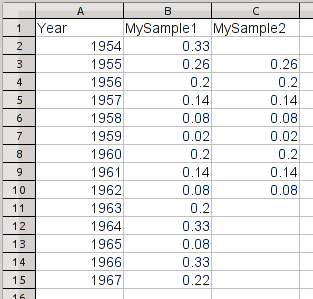
\includegraphics[width=4cm]{excel.png}
\index{File formats!Microsoft Excel 97/2000/XP|)}



\chapter{Microsoft Excel 2007}
\index{File formats!Microsoft Excel 2007|(}
\index{File formats!Office Open XML Spreadsheet|see{Microsoft Excel 2007}}
\index{File formats!OOXML|see{Microsoft Excel 2007}}
\index{File formats!OpenXML Spreadsheet|see{Microsoft Excel 2007}}
\begin{table*}[htbp]
\label{summary:ooxml}
\begin{center}
\begin{tabular*}{15cm}{ l @{\extracolsep{\fill}} p{9cm} }
  \toprule

Format name     	 & Microsoft Excel 2007 \\
Other name(s)      	 & Office Open XML Spreadsheet, OOXML, OpenXML\\
Type      	 	 & XML file\\
Extension(s)      	 & xlsx\\
Read/write support     	 & Read and write \\
Reference implementation & ISO 29500\\
Data / metadata      	 & Data only\\
Calendar type		 & Gregorian\\
Absolute dating support	 & Yes\\
Undated series support   & No\\
Relative dating support  & No\\
Multi series support	 & Yes\\
Original designer	 & Microsoft\\

\bottomrule
\end{tabular*}
\end{center}
\end{table*}

\section{Description}
This is the new XML file format introduced by Microsoft with Excel 2007. Unlike the binary format used by the previous version of Excel, this format is an open standard. However, it should not be confused with the OpenDocument Format standard that was developed by the OASIS consortium.

The layout of the data sheet should be just as for the Excel 97/2000/XP format:

\begin{itemize*}
 \item Row 1 - Header names for each column
 \item Column A - Year values
 \item Column B+ - One column for each series containing data values. Cells are left empty if no data is available for a series because it does not extend to a particular year. Data must be continuous for each series, so missing/unmeasured rings should be included as zero.
\end{itemize*}

See the screenshot in the Microsoft Excel 97/2000/XP format to see how an example of how the spreadsheet should look.
\index{File formats!Microsoft Excel 2007|)}



\chapter{Nottingham}
\index{File formats!Nottingham|(}
\begin{table*}[htbp]
\label{summary:nottingham}
\begin{center}
\begin{tabular*}{15cm}{ l @{\extracolsep{\fill}} p{9cm} }
  \toprule

Format name     	 & Nottingham\\
Other name(s)      	 & Nottingham Laboratory format\\
Type      	 	 & Text file\\
Extension(s)      	 & txt\\
Read/write support     	 & Read and write\\
Reference implementation & Unknown\\
Data / metadata      	 & Data only\\
Calendar type		 & n/a\\
Absolute dating support	 & No\\
Undated series support   & Yes\\
Relative dating support  & No\\
Multi series support	 & Yes\\
Original designer	 & Cliff Litton\\

\bottomrule
\end{tabular*}
\end{center}
\end{table*}

\section{Description}

The Nottingham format was designed by Cliff Litton. It is a simple text format with no support for metadata.

Line 1 contains a series name and an integer indicating how many data values there are in the file. Subsequent lines contain the data represented as 1/100th mm integers in twenty columns seemingly in either 4 characters or 3 characters + 1 space.

There is no known reference implementation for this format and few known examples of data so little is known about how it should handle unusual situations such as negative values, values >999 etc. 

\newpage
\section{Example file}

\begin{lstlisting}
 ABCD01    176
 342 338 334 409 362 308 360 264 325 318 134 151 219 268 290 222 278 258 173 198
 294 202 170 176 172 121  87 130 114 108 170 135 131 126  87 100  86 104 103 127
 112  94  96 120 168 149 119 124  79  67  88  90  93  77  49  42  53  38  57  43
  50  41  56  66  62  55  55  45  47  63  58  60  44  45  49  50  62  61  43  54
  91  60  56  43  52  51  65  68  55  44  41  75  94  78  63  69  58  75  55  47
  58  46  62  45  52  50  77  50  63  75  77  64  66  57  80  57  78  65  68  75
  65  98  85  82 119  89  85  87  83 108 129 123 160 117 129 121  88  69  97  77
  96 106  71  89  50  65 133  89  88  50  60  95  95  91 102 158  83  55  98  70
  45  46  40  36  64  58  52  58  56  94  51  48  47  60  49  48
\end{lstlisting}
\index{File formats!Nottingham|)}

\chapter{ODF Spreadsheet}
\index{File formats!ODF Spreadsheet|(}
\index{File formats!OpenDocument Format|see{ODF Spreadsheet}}
\index{File formats!OpenOffice.org Format|see{ODF Spreadsheet}}
\begin{table*}[htbp]
\label{summary:odfmatrix}
\begin{center}
\begin{tabular*}{15cm}{ l @{\extracolsep{\fill}} p{9cm} }
  \toprule

Format name     	 & ODF Spreadsheet\\
Other name(s)      	 & ODF, ODS, OpenDocument Spreadsheet, OpenOffice.org Spreadsheet, \\
Type      	 	 & XML file\\
Extension(s)      	 & ods \\
Read/write support     	 & Read and write\\
Reference implementation & ISO/IEC 26300:2006 \\
Data / metadata      	 & Data only\\
Calendar type		 & Gregorian\\
Absolute dating support	 & Yes\\
Undated series support   & No \\
Relative dating support  & No \\
Multi series support	 & Yes \\
Original designer	 & OASIS consortium\\

\bottomrule
\end{tabular*}
\end{center}
\end{table*}

\section{Description}

The OpenDocument Format (ODF) spreadsheet format is an XML-based specification developed by the Organization for the Advancement of Structured Information Standards (OASIS) consortium.  It should not be confused with the similarly named Office Open XML format developed by Microsoft.  The ODF spreadsheet format is an open standard which can be read by most modern spreadsheet applications including MS Excel, OpenOffice.org and Google Docs.

Support for ODF spreadsheets in TRiCYCLE is necessarily limited to a particular layout of spreadsheet:

\begin{itemize*}
 \item Row 1 - Header names for each column
 \item Column A - Year values
 \item Column B+ - One column for each series containing data values. Cells are left empty if no data is available for a series because it does not extend to a particular year. Data must be continuous for each series, so missing/unmeasured rings should be included as zero.
\end{itemize*}

Please see the Excel section for a screenshot of how an ODF spreadsheet should look.
\index{File formats!ODF Spreadsheet|)}



\chapter{Oxford}
\index{File formats!Oxford|(}
\begin{table*}[htbp]
\label{summary:oxford}
\begin{center}
\begin{tabular*}{15cm}{ l @{\extracolsep{\fill}} p{9cm} }
  \toprule

Format name     	 & Oxford\\
Other name(s)      	 & Dan Miles Format, English Heritage Format\\
Type      	 	 & Text file\\
Extension(s)      	 & Various including dan, ddf but often none\\
Read/write support     	 & Read and write\\
Reference implementation & Various English Heritage applications\\
Data / metadata      	 & Data only\\
Calendar type		 & Gregorian\\
Absolute dating support	 & Yes\\
Undated series support   & Yes\\
Relative dating support  & Yes\\
Multi series support	 & No\\
Original designer	 & Ancient Monuments Laboratory of English Heritage\\

\bottomrule
\end{tabular*}
\end{center}
\end{table*}

\section{Description}

The Oxford format seems to be only currently used in the Oxford Dendrochronology Laboratory. It was designed in the 1980s for use with a number of DOS based applications for the English Heritage Ancient Monuments Laboratory. It is still actively used by the Oxford Lab with these programs and a number of newer Windows applications.

The file is a text file format containing two header lines following by a block of data values and an optional block of count/sample depth values. Some files also contain a number of comment lines at the end of the file.

Line 1 contains the following fields: 

\begin{itemize*}
 \item Char 1 - Apostrophe
 \item Chars 2-8 - Series name
 \item Char 9-10 - spaces
 \item Char 11 - <
 \item Chars 12-15 - First year in sequence (when series is securely dated).  Year should be left padded with spaces if less than 4 characters.
 \item Char 16 - hyphen
 \item Chars 17-20 - Last year in sequence (when series is securely dated).  Year should be left padded with spaces if less than 4 characters.
 \item Char 21 - space
 \item Char 22+ - Description - typically name of site/building etc
 \item Final char - optional apostrophe 
\end{itemize*}

Line 2 contains:

\begin{itemize*}
 \item Integer number of years
 \item Comma
 \item Integer start year
\end{itemize*}


The start year on line 2 and the first year on line 1 will be the same for securely dated series. When the series is tentatively or relatively dated the first year (and/or) the last year on line 1 will be left blank. For undated series the start year is set to 1001.

The data lines follow the two header lines. These typically contain 10 data values per line, but there can be more (if rings have been added) or less e.g. last line. The values are in 1/100th mm integers and can only contain three digits (e.g. max 999 1/100th mm). Data values are space delimited. Some example files contain values that are left padded with zeros if the value is on 1 or 2 characters wide (e.g. '025' rather than ' 25').

Following the data values there should be an empty line followed by an optional sample count/depth block. The count block is formatted in largely the same way as the data values block. The values are stored in columns 2 characters (rather than 3 characters) wide. Like the data values, the count values are space delimited integers, typically (but not always) 10 per line.

The file is terminated with 0, 1 or 2 free-text comment lines. A number of Oxford data files have been seen that terminate with the ASCII control character referred to variably as 'SUB', 'SUBSTITUTE' or 'CTRL+Z' (represented in Unicode as character dec 26 - hex 1A). It is not clear whether this is necessary for any particular programs to function. 

\section{Limitations}

\begin{itemize*}
 \item Only holds whole ring-width data
 \item Does not cope with data values >999 1/100th mm
 \item Does not cope with chronologies of >99 samples
 \item Does not allow dates before 1AD
\end{itemize*}

\newpage
\section{Example file}

\begin{lstlisting}
'ABCD      <1850-1925> A Fictious site - abcd1 abcd2'
75,1850 
422 582 355 266 225 271 361 235 387 395 
794 611 446 248 277 359 111 226 189 711 
464 172 190 239 128 153 234 828 207 157 
768 180 178 168 204 163 160 255 166 136 
182 201 142 188 223 186 150 135 134 666 
191 122 223 555 123 126 108 133 137 134 
161 222  93 100 132 104  86 277 101 141 
185 151 261 110 145 

  1  2  2  2  2  2  2  2  2  2
  2  2  2  2  2  2  2  2  2  2
  2  2  2  2  2  2  2  2  2  2
  2  2  2  2  2  2  2  2  2  2
  2  2  2  2  2  2  2  2  2  2
  2  2  2  2  2  2  2  2  2  2
  2  2  2  2  2  2  2  2  2  2
  2  2  2  2  1
\end{lstlisting}
\index{File formats!Oxford|)}


\chapter{PAST4}
\index{File formats!PAST4|(}
\begin{table*}[htbp]
\label{summary:past4}
\begin{center}
\begin{tabular*}{15cm}{ l @{\extracolsep{\fill}} p{9cm} }
  \toprule

Format name     	 & PAST4\\
Other name(s)      	 & P4P PAST4 Project File\\
Type      	 	 & Text file\\
Extension(s)      	 & p4p\\
Read/write support     	 & Read and write\\
Reference implementation & PAST4\\
Data / metadata      	 & Data and some structured metadata\\
Calendar type		 & Gregorian\\
Absolute dating support	 & Yes\\
Undated series support   & \\
Relative dating support  & \\
Multi series support	 & Yes\\
Original designer	 & Bernhard Knibbe \\

\bottomrule
\end{tabular*}
\end{center}
\end{table*}

The PAST4 format \citep{past} is the native file format for SCIEM's PAST4 software. It is a hybrid XML file, containing most metadata in structured XML but some metadata and all data as plain text. It is unique amongst dendro data formats in that it contains not only data and metadata but also settings information for the PAST4 software such as details on what colours to use in graphs, which series should be displayed on screen etc. The general structure of a P4P file is as follows:

\begin{itemize*}
    \item  Project header (required)
    \item  Settings (optional)
    \item  Groups (required, repeatable)
    \item  Records (required, repeatable) 
\end{itemize*}


The root XML tag for the file is \verb|<PAST_4_PROJECT_FILE>|. Inside this is the \verb|<PROJECT>| tag which contains the following attributes:

\begin{itemize*}
    \item  ActiveGroup - Zero based index specifying which group is active
    \item  EditDate - Date the file was last edited
    \item  Groups - Number of groups within this project
    \item  Locked - Either TRUE or FALSE indicating whether a password is required to open the file
    \item  Name - Name of the project
    \item  Password - Password used to lock the project
    \item  PersID - Abbreviation of the authors name
    \item  Records - Number of records in the project
    \item  Reference - Zero based index indicated which is the reference series (-1 if none selected)
    \item  Sample - Zero based index indicating which is the selected sample (-1 if none selected)
    \item  Version - Version number for this PAST4 format. At the time of writing only one version exists (400). 
\end{itemize*}

Of these fields only Name, Groups and Records are mandatory. The project tag can also contain a \verb|<![CDATA[| tag which allows the storing of a project description in plain text.

Next comes the \verb|<SETTINGS>| tag. This is one very large XML tag with many attributes controlling the what PAST4 should display the data. The contents of this tag are optional and are therefore irrelevant for the transfer of dendro data.

Next comes one or more \verb|<GROUPS>| tags. A group is an arbitrary collection of series, perhaps representing a number of measurements of a single object, or perhaps an administrative collection of series. Groups can be nested in a hierarchy, but rather than use the hierarchical nature of XML files, the format instead lists all groups side-by-side and maintains the relationships through the use of an 'owner' attribute containing the index of the parent group. This arrangement means than any changes to the hierarchy, or the deletion of a group requires all indices to be carefully updated to avoid corrupting the file. The group tag has the following attributes:

\begin{itemize*}
    \item  Name - Name of the group
    \item  Visible - Either TRUE or FALSE indicating whether the group should be shown in graphs
    \item  Fixed - Either TRUE or FALSE indicating whether the group can be moved
    \item  Locked - Either TRUE or FALSE. If locked the group can be used in the calculation of further mean values.
    \item  Changed - Internal TRUE or FALSE value for keeping track of changes
    \item  Expanded - TRUE or FALSE value indicating whether the group should be expanding in the project navigator window
    \item  UseColor - TRUE or FALSE value for is content should be displayed in color
    \item  HasMeanValue - TRUE or FALSE indicating if the group has a dynamic mean value
    \item  IsChrono - TRUE or FALSE indicating if the group mean is calculated with sample depth information
    \item  Checked - TRUE or FALSE indicating if the group is locked and checked
    \item  Selected - TRUE or FALSE indicated in the group is selected in the project navigation window
    \item  Color - 24bit integer indicating the RGB volor value for the group using Borland format
    \item  Quality - Integer value describing the quality of the group mean
    \item  MVKeycode - String code for the group. If empty the Name field is used
    \item  Owner - Integer pointing containing the index of the parent group if this group is in a hierarchy. If its a top level group it should be -1. 
\end{itemize*}

As with the project tag, the group tag can also contain a \verb|<![CDATA[| section for storing a plain text description of the group.

The final tag type in the file is the \verb|<RECORDS>| tag. These contain the actual data series and most of the metadata. Like group tags, records tags are placed side-by-side in the file and are placed into the group hierarchy by the use of the 'owner' attribute. In addition, the tag also has the following attributes:

\begin{itemize*}
    \item  Keycode - Name of the series
    \item  Length - Integer for the number of rings
    \item  Owner - Integer index to the group to which this record belongs
    \item  Chrono - TRUE or FALSE indicating whether this record has density information
    \item  Locked - TRUE or FALSE indicating in the record can be moved
    \item  Filter - TRUE or FALSE indicating if an indexing function is appled to the data
    \item  FilterIndex - Integer index for the filter used
    \item  FilterS1 - Parameter 1 for the filter
    \item  FilterS2 - Parameter 2 for the filter
    \item  FilterB1 - Additional filter parameter
    \item  FilterWeight - Additional filter parameter
    \item  Offset - Position of the first ring
    \item  Color - 24bit RGB color for record in Borland format
    \item  Checked - TRUE or FALSE indicating is the record is selected for use in the dynamic group mean
    \item  !VShift - Temporary integer value added to data value to shift vertically in graphs
    \item  IsMeanValue - TRUE or FALSE indicating if this is a dynamic mean value
    \item  Pith - TRUE or FALSE
    \item  SapWood - Integer storing the number of sapwood rings
    \item  Location - String location information
    \item  Waldkante - String description of presence of waney edge
    \item  FirstValidRing - Integer indicating which ring is the first valid ring. If >0 then some rings are discarded
    \item  LastValidRing - Integer indicating which ring is the last valid ring. If >0 then some rings are discarded
    \item  UseValidRingsOnly - TRUE or FALSE - internal use only
    \item  Quality - Integer indicating the quality of the record 
\end{itemize*}
The record tag then contains a \verb|<HEADER>| tag with a \verb|<![CDATA[| section which includes additional free-text header information. There are no requirements as to how information should be laid out in this field however many users seem to adopt the Heidelberg style of keyword=value.

Next comes the \verb|<DATA>| tag which is empty except another \verb|<![CDATA[| section. This is where the actual ring-width data is stored. Each data value is recorded on a separate line (using CR LR line breaks). Each line contains the following six tab delimited fields:

\begin{itemize*}
    \item  Ring width as a floating point number
    \item  Sample depth
    \item  Number of sample increasing
    \item  Latewood percentage as a floating point value 0-1 (0 if not known)
    \item  Duplicate/backup ring-width value to store the original ring-width value. If an index is applied the ring-width value in column 1 is altered.
    \item  Comment string about this particular ring 
\end{itemize*}

\section{Dating}

PAST4 contains an option for enabling/disabling the year 0 but it does not record within the data file whether the option was set when the file was created. By default the year 0 is disabled therefore the library treats PAST4 files as if they use the Gregorian calendar but it is possible that files were in fact created with the Astronomical calendar in mind. 

\newpage
\section{Example file}
\begin{lstlisting}
<?xml version="1.0"?>
<PAST_4_PROJECT_FILE>
    <PROJECT Name="title0" Version="400" Locked="FALSE" Password=""
        CreationDate="04/05/2006 2:13:51 PM" EditDate="09/01/2010 13:02" ActiveGroup="0"
        Reference="-1" Sample="-1" PersID="investigator0" Groups="2" Records="3">
<![CDATA[description0
]]></PROJECT>
    <SETTINGS/>
    <GROUP Name="title1" Visible="TRUE" Fixed="FALSE" Locked="FALSE" Changed="FALSE" 
	Expanded="TRUE" UseColor="TRUE" HasMeanValue="FALSE" IsChrono="FALSE" 
	Checked="FALSE" Selected="FALSE" Color="0" MVKeycode="" Owner="-1">
	<![CDATA[]]></GROUP>
    <GROUP Name="Unnamed Group" Visible="TRUE" Fixed="FALSE" Locked="FALSE" Changed="FALSE"
        Expanded="TRUE" UseColor="TRUE" HasMeanValue="FALSE" IsChrono="FALSE" Checked="FALSE"
        Selected="FALSE" Color="0" MVKeycode="" Owner="-1"><![CDATA[]]></GROUP>
    <RECORD Keycode="title6" Length="4" Owner="0" Chrono="FALSE" Locked="FALSE" Filter="FALSE"
        FilterIndex="-1" FilterS1="100" FilterS2="100" FilterB1="FALSE" FilterWeight="" Offset="0"
        Color="0" Checked="FALSE" VShift="0" IsMeanValue="0" Pith="FALSE" SapWood="0"
        Location="locationComment1" Species="Quercus" Waldkante="" FirstValidRing="0"
        LastValidRing="0" UseValidRingsOnly="FALSE">
        <HEADER><![CDATA[Unit=1/100th millimetres
]]></HEADER>
        <DATA><![CDATA[123      1       1       0       123     
123     1       1       0       123     
123     1       1       0       123     
125     1       1       0       125     
]]></DATA>
    </RECORD>
    <RECORD Keycode="title6" Length="4" Owner="0" Chrono="FALSE" Locked="FALSE" Filter="FALSE"
        FilterIndex="-1" FilterS1="100" FilterS2="100" FilterB1="FALSE" FilterWeight="" Offset="0"
        Color="0" Checked="FALSE" VShift="0" IsMeanValue="0" Pith="FALSE" SapWood="0"
        Location="locationComment1" Species="QUSP" Waldkante="" FirstValidRing="0"
        LastValidRing="0" UseValidRingsOnly="FALSE">
        <HEADER><![CDATA[Unit=1/100th millimetres
]]></HEADER>
        <DATA><![CDATA[123      1       1       0       123     
123     1       1       0       123     
123     1       1       0       123     
125     1       1       0       125     
]]></DATA>
    </RECORD>
    <RECORD Keycode="Unnamed series" Length="2" Owner="1" Chrono="FALSE" Locked="FALSE"
        Filter="FALSE" FilterIndex="-1" FilterS1="100" FilterS2="100" FilterB1="FALSE"
        FilterWeight="" Offset="0" Color="0" Checked="FALSE" VShift="0" IsMeanValue="0" 
	Pith="FALSE" SapWood="0" Location="" Species="" Waldkante="" FirstValidRing="0" 
	LastValidRing="0" UseValidRingsOnly="FALSE">
        <HEADER><![CDATA[Unit=Wierd units
]]></HEADER>
        <DATA><![CDATA[96       1       1       0       96      fire_damage; fire_damage; 
34      1       1       0       34      fire_damage; fire_damage; 
]]></DATA>
    </RECORD>
</PAST_4_PROJECT_FILE>
\end{lstlisting}
\index{File formats!PAST4|)}

\chapter{Sheffield}
\index{File formats!Sheffield|(}
\index{File formats!D Format|see{Sheffield}}
\begin{table*}[htbp]
\label{summary:sheffield}
\begin{center}
\begin{tabular*}{15cm}{ l @{\extracolsep{\fill}} p{9cm} }
  \toprule

Format name     	 & Sheffield\\
Other name(s)      	 & D Format\\
Type      	 	 & Text file\\
Extension(s)      	 & .d\\
Read/write support     	 & Read and write\\
Reference implementation & Dendro for Windows\\
Data / metadata      	 & Data and some structured metadata\\
Calendar type		 & Gregorian\\
Absolute dating support	 & Yes\\
Undated series support   & No\\
Relative dating support  & Yes\\
Multi series support	 & No\\
Original designer	 & Ian Tyers\\

\bottomrule
\end{tabular*}
\end{center}
\end{table*}

\section{Description}

Sheffield format \citep{dendroforwin} is a dendro specific text file designed by Ian Tyers for his Dendro for Windows application. It is probably most widely used in the UK but is also used in continental Europe as well as New Zealand.

The format contains both data and some structured metadata with each field/value stored one per line. The order of fields is fixed so missing data must be indicated by the use of a question mark. The data present on each line is as follows:

\begin{enumerate*}
 \item Site name/sample number - Free form text not including \verb|,"()| up to 64 characters 
 \item Number of rings - Whole positive number 
 \item Date type - Single character; A = absolute date, R = relative date 
 \item Start date - Whole number (can be negative).  If absolute year then add 10000 to value so 1AD = 10001
 \item Raw data type \emph{or} Mean data type 
      \begin{itemize*}   
       \item Single character; R = annual raw ring-width data (NB earlier versions used some other codes here for species e.g. ABEFPSU these are all interpreted as equivalent to R) 
       \item Single character; W=timber mean with signatures, X=chron mean with signatures, T = timber mean, C = chron mean, M = un-weighted master sequence 
      \end{itemize*} 
 \item Raw sapwood number \emph{or} mean number of timbers/chronologies
      \begin{itemize*}   
       \item Whole positive number or 0 
       \item Whole positive number
      \end{itemize*} 
 \item Raw edges inf. \emph{or} Mean chronology type
      \begin{itemize*}   
       \item Single character; Y = has bark, ! = has ?bark, W = terminal ring probably complete (i.e. possibly Winter Felled), S = terminal ring probably incomplete (i.e. possibly Summer Felled), B = has h/s boundary, ? = has ?h/s boundary, N = has no specific edge, (NB but may have sap), U = sap/bark unknown, C = charred outer edge, P = possibly charred outer edge 
       \item Single character; R = raw unfiltered data, 5 = 5 year running mean, I = indexed data, U = unknown mean type 
      \end{itemize*} 
 \item Author and comment - Free form text not including \verb|,"()| up to 64 characters 
 \item UK National grid reference - 2 characters +even no of digits up to 14 characters in all, ? = not known e.g. TQ67848675
 \item Latitude and longitude - Either decimal format e.g. 53.382457;-1.513623 or previously N51\verb|^|30 W1\verb|^|20
 \item Pith - single character; C = centre of tree, V = within 5 years of centre, F = 5-10 years of centre, G = greater than 10, ? = unknown
 \item Cross-section code - Two character code; first character, A = whole roundwood, B = half round, C quartered, D radial/split plank, E tangential/sawn plank. second character, 1 untrimmed, 2 trimmed, X irregularly trimmed. or, X = core /unclassifiable, ? unknown/unrecorded 
 \item Major dimension - whole number in mm, 0 if unrecorded or mean
 \item Minor dimension - whole number in mm, 0 if unrecorded or mean
 \item Unmeasured inner rings - single character+whole number; use pith codes + number of rings or, H = heartwood, N = none 
 \item Unmeasured outer rings - single character+whole number; use edges code + number of rings except that S = sapwood with no edge and V is the spring felling equivalent other codes are, H = heartwood with no edge, N = none
 \item Group/Phase - free form text not including , " ( ) up to 14 characters 
 \item Short title - free form text not including , " ( ) up to 8 characters 
 \item Period - single character; C = modern, P = post medieval, M = medieval, S = Saxon, R = Roman, A = pre Roman, 2 = duplicate e.g. repeat measure, B = multiperiod e.g. long master, ? = unknown 
 \item ITRDB species code - 4 character code - refer to ITRDB species codes 
 \item Interpretation and anatomical notes - ? =no interpretation/notes. The interpretation and the anatomical notes can be in any order but each must consist of three parts, a single character A or I for anatomy or interpretation, a separator ~, for interpretations the date of the start, for anatomy the ringno, a separator ~, for anatomy the anatomical code for interpretations P for plus, 0 for felled and a number for the length of the range, where more than one record is present these are separated by ~, there must not be a terminal separator and each record must consist of the tree parts. The anatomical codings can be anything of a single character but supported usage is based on Hans-Hubert Leuschners anatomical codes; D = Density Band, R = Reaction Wood, L = Light Latewood, H = Dense Latewood, F = Frost Ring, K = Small Earlywood Vessels - oak, G = Great Latewood Vessels - oak, T = Wound Tissue, N = Narrow Latewood, A = Light Latewood End, P = Narrow and Light Latewood, Q = Narrow and Dense Latewood 
 \item Data type - single character; D = ring widths, E = early-wood widths only, L = late-wood widths only, R = late+early wood widths (i.e. reverse of normal rings), I = minimum density, A = maximum density, S = early, late; (i.e. sequentially and separately), M = mixed (?means of others)

\end{enumerate*}

The remaining lines contain the data:

\begin{itemize*}
 \item For each width (equivalent to the value of length) the individual increments etc. if a C X T or W type mean.  No negatives or zeros
 \item Check field - Single character H
 \item For each width the individual weightings of the mean sequences. If an X or W type mean.  No negatives or zeros.
 \item Check field - Single character R
 \item For each width the number of individual series with rising values.  No negatives or zeros.
 \item Check field - Single character F
 \item For each width the number of individual series with falling values. No negatives.
\end{itemize*}

\section{Dating}

The format copes with the problem of the non-existent year 0AD/BC by adding 10000 to all year values. Therefore: 

\begin{table*}[htbp]
\begin{center}
\begin{tabular*}{5cm}{l @{\extracolsep{\fill}} l}
\toprule
Year & Value in file\\
\midrule
1AD & 10001\\
1BC & 10000\\
9999BC & 2\\
10000BC & 1\\
\bottomrule
\end{tabular*}
\end{center}
\end{table*}

\section{Example file}
\begin{lstlisting}
Ship wreck 4 timber mean
170
A
10784
W
4
R
made PB 22/6/2004
?
?
?
?
0
0
N
N
A
Example
M
QUSP
?
D
391
454
309
314
270
273
229
319
267
276
128
163
221
269
214
201
218
199
198
209
156
177
...
\end{lstlisting}
\index{File formats!Sheffield|)}


\chapter{Topham}
\index{File formats!Topham|(}
\begin{table*}[htbp]
\label{summary:topham}
\begin{center}
\begin{tabular*}{15cm}{ l @{\extracolsep{\fill}} p{9cm} }
  \toprule

Format name     	 & Topham\\
Other name(s)      	 & Instrument format\\
Type      	 	 & Text file\\
Extension(s)      	 & txt\\
Read/write support     	 & Read and write\\
Reference implementation & \\
Data / metadata      	 & Data only\\
Calendar type		 & n/a\\
Absolute dating support	 & No\\
Undated series support   & Yes\\
Relative dating support  & No\\
Multi series support	 & No\\
Original designer	 & John Topham\\

\bottomrule
\end{tabular*}
\end{center}
\end{table*}

\section{Description}

The Topham format is probably the most simplistic of formats consisting of just a column of decimal data values and no metadata whatsoever. Each data value is a decimal ring width in millimetres. 

\section{Example file}

\begin{lstlisting}
3.42
3.38
3.34
4.09
3.62
3.08
3.60
2.64
3.25
3.18
3.42
3.38
...
\end{lstlisting}


\chapter{TRiDaS}
\index{File formats!TRiDaS|(}
\index{TRiDaS|(}
\begin{table*}[htbp]
\label{summary:tridas}
\begin{center}
\begin{tabular*}{15cm}{ l @{\extracolsep{\fill}} p{9cm} }
  \toprule

Format name     	 & TRiDaS\\
Other name(s)      	 & Tree-Ring Data Standard, TRiDaS XML\\
Type      	 	 & Text file\\
Extension(s)      	 & xml\\
Read/write support     	 & Read and write\\
Reference implementation & TRiCYCLE\\
Data / metadata      	 & Data and structured metadata\\
Calendar type		 & Gregorian\\
Absolute dating support	 & Yes\\
Undated series support   & Yes\\
Relative dating support  & Yes\\
Multi series support	 & Yes\\
Original designer	 & Esther Jansma, Peter Brewer and Ivo Zandhuis\\

\bottomrule
\end{tabular*}
\end{center}
\end{table*}

\section{Description}

TRiDaS (Tree-Ring Data Standard see \url{http://www.tridas.org}) is a data format designed by over 80 dendrochronologists, computer scientists and users of dendrochronological data from a variety of associated fields as part of the DCCD project and the Dendro Data Standard forum. It is designed to accurately represent any dendro data and metadata and it is hoped over time the dendro community will accept TRiDaS as the de facto standard for all dendro data.

The format uses extensible markup language (XML) which means the standard can be extended and evolve as future needs change. The format is structured around the eight data entities described below: 

\begin{description*}

\item[A project] is defined by a laboratory and encompasses dendrochronological research of a particular object or group of objects. Examples include: the dating of a building; the research of forest dynamics in a stand of living trees; the dating of all Rembrandt paintings in a museum. What is considered a “project” is up to the laboratory performing the research. It could be the dating of a group of objects, but the laboratory can also decide to define a separate project for each object. Therefore, a project can have one or more objects associated with it.

\item[An object] is the item to be investigated. Examples include: violin; excavation site; painting on a wooden panel; water well; church; carving; ship; forest. An object could also be more specific, for example: mast of a ship; roof of a church. Depending on the object type various descriptions are made possible. An object can have one or more elements and can also refer to another (sub) object. For instance a single file may contain three objects: an archaeological site object, within which there is a building object, within which there is a beam object. The list of possible object types is extensible and is thus flexible enough to incorporate the diversity of data required by the dendro community. Only information that is essential for dendrochronological research is recorded here. Other related data may be provided in the form of a link to an external database such as a museum catalogue.

\item[An element] is a piece of wood originating from a single tree. Examples include: one plank of a water well; a single wooden panel in a painting; the left-hand back plate of a violin; one beam in a roof; a tree trunk preserved in the soil; a living tree. The element is a specific part of exactly one object or sub object. An object will often consist of more than one element, e.g., when dealing with the staves (elements) of a barrel (object). One or more samples can be taken from an element and an element may be dated using one or more derivedSeries.

\item[A sample] is a physical specimen or non-physical representation of an element. Examples include: core from a living tree; core from a rafter in a church roof; piece of charcoal from an archaeological trench; slice from a pile used in a pile foundation; wax imprint of the outer end of a plank; photo of a back plate of a string instrument. Note that a sample always exists and that it can either be physical (e.g. a core) or representative (e.g. a picture). A sample is taken from exactly one element and can be represented by one or more radii.

\item[A radius] is a line from pith to bark along which the measurements are taken. A radius is derived from exactly one sample. It can be measured more than once resulting in multiple measurementSeries.

\item[A measurementSeries] is a series of direct, raw measurements along a radius. A single measurementSeries can be standardised or a collection of measurementSeries can be combined into a derived- Series. The measurements themselves are stored separately as values.

\item[A derivedSeries] is a calculated series of values and is a minor modification of the “v-series” concept proposed by \citet{corina}. Examples include: index; average of a collection of measurementSeries such as a chronology. A derivedSeries is derived from one or more measurementSeries and has multiple values associated with it.

\item[A value] is the result of a single ring measurement. Examples include: total ring width; earlywood width; latewood width. The values are related to a measurementSeries or a derivedSeries. In case of a measurementSeries the variable and its measurement unit (e.g. microns, 1/100th mm etc) are recorded as well. 
\end{description*}

For a full description of the standard see \citet{tridas}.

\section{Example file}
\begin{lstlisting}[language=XML]
<?xml version="1.0" encoding="UTF-8"?>
<tridas xmlns:xsi="http://www.w3.org/2001/XMLSchema-instance"
    xsi:schemaLocation="http://www.tridas.org/1.2.1 ../dev/sourceforge/tridas/XMLSchema/1.2.1/tridas-1.2.1.xsd"
    xmlns="http://www.tridas.org/1.2.1" xmlns:xlink="http://www.w3.org/1999/xlink">
    <project>
        <title>Aegean Dendrochronology Project</title>
        <identifier domain="dendro.cornell.edu">C</identifier>
        <createdTimestamp certainty="exact">1997-02-01T14:13:51.0Z</createdTimestamp>
        <lastModifiedTimestamp certainty="exact">1997-02-01T14:13:51.0Z</lastModifiedTimestamp>
        <type>Dating</type>
        <description>Our key long-range goal is to build long multi-millennial scale tree-ring
            chronologies in the Aegean and Near East that will extend from the present to the 
	    early Holocene to cover, broadly speaking, the last 10,000 years of human and 
	    environmental history. Our raison d'etre is to provide a dating method for the study
	    of history and prehistory in the Aegean that is accurate to the year. This kind of 
	    precision has, up to now, been lacking in ancient studies of this area. Indeed, few 
	    archaeological problems stimulate as much rancor as chronology, especially that of 
	    the Eastern Mediterranean. The work of the Aegean and Near Eastern Dendrochronology 
	    Project aims to help to bring some kind of rational and neutral order to Aegean and 
	    Near Eastern chronology from the Neolithic to the present. </description>
        <laboratory>
            <name>Malcolm and Carolyn Weiner Laboratory for Aegean and Near Eastern Dendrochronology</name>
            <address>
                <addressLine1>B48 Goldwin Smith Hall</addressLine1>
                <addressLine2>Cornell University</addressLine2>
                <cityOrTown>Ithaca</cityOrTown>
                <stateProvinceRegion>NY</stateProvinceRegion>
                <postalCode>14853</postalCode>
                <country>USA</country>
            </address>
        </laboratory>
        <category>Archaeology</category>
        <investigator>Peter I Kuniholm</investigator>
        <period>1976-present</period>
        <reference>reference1</reference>
        <object>
            <title>White Tower, Thessaloniki</title>
            <identifier domain="dendro.cornell.edu"
                >28acb483-f337-412f-a063-59d911c37594</identifier>
            <createdTimestamp certainty="exact">1997-02-01T14:13:51.0Z</createdTimestamp>
            <lastModifiedTimestamp certainty="exact">1997-02-01T14:13:51.0Z</lastModifiedTimestamp>
            <type normalStd="Corina Dictionary" normalId="4" normal="Building">Building</type>
            <description>The White Tower of Thessaloniki was originally constructed by the Ottomans
                to fortify the city's harbour.</description>
            <coverage>
                <coverageTemporal>Ottoman</coverageTemporal>
                <coverageTemporalFoundation>Stylistic</coverageTemporalFoundation>
            </coverage>
            <location>
                <locationGeometry xmlns:gml="http://www.opengis.net/gml">
                    <gml:Point srsName="urn:ogc:def:crs:EPSG:6.6:4326">
                        <gml:pos>40.6263 22.9485</gml:pos>
                    </gml:Point>
                </locationGeometry>
                <locationPrecision>20</locationPrecision>
                <locationComment>Thessaloniki, Greece</locationComment>
            </location>
            <object>
                <title>Fourth floor</title>
                <type>Floor</type>
                <element>
                    <title>C-TWT-65</title>
                    <identifier domain="dendro.cornell.edu"
                        >89dbd409-03a3-42a0-9391-62c6be7009ad</identifier>
                    <createdTimestamp certainty="exact">1997-02-01T14:13:51.0Z</createdTimestamp>
                    <lastModifiedTimestamp certainty="exact"
                        >1997-02-01T14:13:51.0Z</lastModifiedTimestamp>
                    <type normalStd="Corina Dictionary" normalId="3" normal="Rafter">Rafter</type>
                    <description>15th Rafter from the south</description>
                    <taxon normalStd="Catalogue of Life Annual Checklist 2008" normal="Quercus"
                        normalId="49139">Quercus sp.</taxon>
                    <dimensions>
                        <unit normalTridas="metres"/>
                        <height>1</height>
                        <width>1</width>
                        <depth>1</depth>
                    </dimensions>
                    <authenticity>Original</authenticity>
                    <sample>
                        <title>C-TWT-65-A</title>
                        <identifier domain="dendro.cornell.edu"
                            >ff688357-b2d4-4394-a21a-90696cd4558c</identifier>
                        <createdTimestamp certainty="exact"
                            >1997-02-01T14:13:51.0Z</createdTimestamp>
                        <lastModifiedTimestamp certainty="exact"
                            >1997-02-01T14:13:51.0Z</lastModifiedTimestamp>
                        <type normal="Corina Dictionary" normalId="1" normalStd="Section"
                            >Section</type>
                        <samplingDate certainty="exact">1981-07-25</samplingDate>
                        <state>Dry</state>
                        <radius>
                            <title>C-TWT-65-A-B</title>
                            <identifier domain="dendro.cornell.edu"
                                >5b7baa8b-cd4e-4b3b-88fa-82939420e544</identifier>
                            <createdTimestamp certainty="exact"
                                >2006-05-04T18:13:51.0Z</createdTimestamp>
                            <lastModifiedTimestamp certainty="exact"
                                >2006-05-04T18:13:51.0Z</lastModifiedTimestamp>
                            <woodCompleteness>
                                <pith presence="absent"/>
                                <heartwood presence="incomplete"/>
                                <sapwood presence="complete"/>
                                <bark presence="present"/>
                            </woodCompleteness>
                            <measurementSeries>
                                <title>C-TWT-65-A-B-A</title>
                                <identifier domain="dendro.cornell.edu"
                                    >8c50234e-8eda-41bb-b578-01cc881d1ea1</identifier>
                                <createdTimestamp certainty="exact"
                                    >1997-02-01T14:13:51.0Z</createdTimestamp>
                                <lastModifiedTimestamp certainty="exact"
                                    >1997-02-01T14:13:51.0Z</lastModifiedTimestamp>
                                <analyst>Laura Steele</analyst>
                                <dendrochronologist>Peter I Kuniholm</dendrochronologist>
                                <measuringMethod normalStd="Corina Dictionary" normalId="1"
                                    >Measuring platform</measuringMethod>
                                <interpretation>
                                    <firstYear suffix="AD">1254</firstYear>
                                    <statFoundation>
                                        <statValue>8.3</statValue>
                                        <type>t-score</type>
                                        <usedSoftware>Corina 2.10</usedSoftware>
                                    </statFoundation>
                                    <deathYear suffix="AD">1535</deathYear>
                                    <provenance>Possibly from the region of Serres</provenance>
                                </interpretation>
                                <values>
                                    <variable normalTridas="Ring width"/>
                                    <unit normalTridas="1/100th millimetres"/>
                                    <value value="54"/>
                                    <value value="111"/>
                                    <value value="71"/>
                                    <value value="40"/>
                                    <value value="56"/>
                                </values>
                            </measurementSeries>
                        </radius>
                    </sample>
                </element>
            </object>
        </object>
    </project>
</tridas>

\end{lstlisting}
\index{TRiDaS|)}
\index{File formats!TRiDaS|)}


\chapter{TRIMS}
\index{File formats!TRIMS|(}
\begin{table*}[htbp]
\label{summary:trims}
\begin{center}
\begin{tabular*}{15cm}{ l @{\extracolsep{\fill}} p{9cm} }
  \toprule

Format name     	 & TRIMS\\
Other name(s)      	 & None known\\
Type      	 	 & Text file\\
Extension(s)      	 & .rw\\
Read/write support     	 & Read and write\\
Reference implementation & \\
Data / metadata      	 & Data only\\
Calendar type		 & Gregorian\\
Absolute dating support	 & Yes\\
Undated series support   & Yes\\
Relative dating support  & No\\
Multi series support	 & No\\
Original designer	 & Unknown\\

\bottomrule
\end{tabular*}
\end{center}
\end{table*}

This is a simple data only text file format. These files were originally produced using the Henson rotary micrometer measuring stages but have largely been phased out. 

\begin{itemize*}
 \item Line 1 - Initials of user that created the series
 \item Line 2 - Date the file was created in dd/MM/YY format
 \item Line 3 - Year of first data value (0 treated as undated series)
 \item Line 4+ - Space character followed by an integer data value in 1/100th mm
 \item Final line - Space character + 999 denoting end of series. 
\end{itemize*}

\section{Example file}
\begin{lstlisting}
pb
05/10/94
 1816 
 169 
 96 
 165 
 85 
 139 
 87 
 112  
 ... 
 999
\end{lstlisting}
\index{File formats!TRIMS|)}


\chapter{Tucson}
\index{File formats!Tucson|(}
\index{File formats!RWL|see{Tucson}}
\index{File formats!CRN|see{Tucson}}
\index{File formats!Decadal|see{Tucson}}
\index{File formats!TSF|see{Tucson}}
\index{File formats!Time series format|see{Tucson}}
\index{File formats!ITRDB|see{Tucson}}
\begin{table*}[htbp]
\label{summary:tucson}
\begin{center}
\begin{tabular*}{15cm}{ l @{\extracolsep{\fill}} p{9cm} }
  \toprule

Format name     	 & Tucson\\
Other name(s)      	 & Decadal, RWL, CRN, ITRDB, Time series format, TSF\\
Type      	 	 & Text file\\
Extension(s)      	 & Various including tuc, rwl, dec, crn\\
Read/write support     	 & Read and write\\
Reference implementation & COFECHA\\
Data / metadata      	 & Data with some structured metadata, however, standardisation of metadata is very poor resulting in metadata often being little more than free text comments\\
Calendar type		 & Astronomical\\
Absolute dating support	 & Yes\\
Undated series support   & No\\
Relative dating support  & No\\
Multi series support	 & Yes\\
Original designer	 & Richard Holmes\\

\bottomrule
\end{tabular*}
\end{center}
\end{table*}

\section{Description}
The Tucson format is perhaps the most widely used dendro data format. Unfortunately it seems there was never definitive documentation. Support for the format has been incorporated into a number of dendro applications but without format documentation there are variations in these implementations resulting in quite a lot of subtle differences in files. The often tight association between the Dendro Program Library (DPL) and the ITRDB means that perhaps the most definitive documentation for the format is the ITRDB website.

The Tucson format is best considered as covering two different sub-formats which are often referred to by their file extensions (RWL and CRN). RWL files are used for storing ring-width data, whereas CRN files are used for storing chronologies.

The ITRDB website includes detailed information on how to include structured metadata in Tucson format files. Unfortunately there are no tools for creating and/or validating Tucson files so the vast majority of files circulating in the community today (including those in the ITRDB) do not adhere to these standards. 

\section{RWL files}
Tucson RWL files begin with three lines of metadata. Strictly these lines should contain structured metadata, but with no software to assist in this, users either only partially stick to these rules, or reject them entirely instead using the three lines as free-text comment lines. The metadata should be set out as follows:

\begin{itemize*}
    \item  Line 1 - Chars 1-6 Site ID
    \item  Line 1 - Chars 10-61 Site Name
    \item  Line 1 - Chars 62-65 Species Code followed by optional ID number
    \item  Line 2 - Chars 1-6 Site ID
    \item  Line 2 - Chars 10-22 State/Country
    \item  Line 2 - Chars 23-30 Species
    \item  Line 2 - Chars 41-45 Elevation
    \item  Line 2 - Chars 48-57 Lat-Long in degrees and minutes, ddmm or dddmm
    \item  Line 2 - Chars 68-76 1st and last Year
    \item  Line 3 - Chars 1-6 Site ID
    \item  Line 3 - Chars 10-72 Lead Investigator
    \item  Line 3 - Chars 73-80 comp. date 
\end{itemize*}

Then follows the data lines which are set out as follows:

\begin{itemize*}
    \item  Chars 1-8 - Series ID - the series ID should be unique in the file so that it is clear where one series ends and another begins when multiple series are present in the same file.
    \item  Next 4 chars - Year of first value in this row.
    \item  Ten data values consisting of a space character and 5 integers. The file and last data line for a series may have less than 10 data values so that the majority of lines begin at the start of a decade.  
\end{itemize*}

The final data value should be followed by a a stop marker which is either 999 or -9999. When a stop marker of 999 is used this indicates that the integer values in the file are measured in 0.01mm (1/100th mm) units, whereas if a -9999 stop marker is used the units are 0.001mm (microns). The stop marker is therefore used to indicate the end of the data series and the units the data are stored in.

There appears to be no official specification as to how missing rings should be encoded, but the standard notation seems to be to use -999 or 0. 

\section{CRN files}

Tucson CRN files are used to store chronology data. In addition to each data values they also have space for a sample depth or count value to record how many values were combined to give each data value. CRN files should strictly begin with the same 3 header lines that are described above for RWL. Like RWL files the specification is often partially adhered to and at times ignored completely.

The data lines for CRN files are quite different to RWL:

\begin{itemize*}
    \item  Chars 1-6 - Series ID
    \item  Next 4 chars - Year of first value in this row.
    \item  Ten data value blocks consisting of four integer characters for the data value, then a space, then two integer characters for sample depth. 
\end{itemize*}

The stop marker in a CRN file should be 9990. 

\section{Workarounds and quirks}

\begin{itemize*}
\item  No information was given as to how to handle the non-existent year 0AD/BC. For data files with years all in the AD period, this is not a problem. Most dendro software seem to treat year numbers in Tucson files as using the 'Astronomical Calendar' whereby 1 = 1AD, 0=1BC, -1=2BC etc. This goes against what most dendrochronologists assume (and do) when using Tucson files. For instance most people that work entirely in the BC period use negative integers to represent BC years e.g. -5 as 5BC. With no clear specification and different people interpreting the format in different ways, there is no way of being certain what data negative year numbers in Tucson files mean.
\item Tucson format places a restriction of just four characters to the year values. This means that strictly the earliest value a Tucson file can represent is -999. Some users work around this by steeling the last character of the series ID to give them five characters for the year. For example: ABCDEFG-9999. This conversely limits the series ID to 7 characters. To add to the confusion, other users have been known to add an arbitrary number (e.g. 5000) to all year numbers to overcome this problem.
\item  The fact that 999 is used as the stop marker for series in 1/100th mm means that Tucson files cannot store a ring value of 9.99mm. In the unlikely event that a sample should have this large a ring, it should be rounded up or down to 998 or 1000.
\item  Some programs appears to add padding values after the stop marker to fill the rest of the 10 data values in the row.
\item  Some data files seem to use 9990 as a stop marker
\item  Some files appears to use a full-stop character to indicate empty data values after the stop marker.
\item  Data values in RWL files are space delimited, however some programs use tabs instead.
\item  When reading Tucson files, COFECHA and ARSTAN ignore all lines that do not match the standard data line format. As such, some users have used this to enable them to include multiple comment lines in their files.
\item  The ITRDB documentation says they should be recorded as DDMM or DDDMM, but this along with sign (N,S,E,W,+ or -) would require 11 characters, when the Tucson specification only allows for 10. Perhaps this was due to an assumption that all places would be in the northern hemisphere? This has resulted in a large amount of variation in the way that coordinates are recorded making it extremely difficult to parse them without error. Here are some examples (including some that use 11 chars not 10): 
\begin{multicols}{2}
\begin{itemize*}
\item  4652N01101E
\item  +4652-01101
\item  N4652E01101
\item  4652-01101
\item  465201101
\item  4652 01101 
\end{itemize*}
\end{multicols}

\end{itemize*}


\section{Example file - raw series}
\begin{lstlisting}
107    1 OBERGURGL
107    2 AUSTRIA      NORWAY SPRUCE      6726  4652N01101E     1911 1959
107    3 GIERTZ                                                 08    76
107011  1911    78    93    43   100    93   110   135   115   102
107011  1920    92   125   110   135    98    80    75   125   102   110
107011  1930   105   105    95   120   135   140   110   120   130   135
107011  1940   120   130   130   165   135   145   155   160    88   135
107011  1950   140   150   140   130   115   130   130   110   110   135
107011  1960   125   120   135   160   15    102   105   135   105   140
107011  1970   120   115   100   110   110   999
107012  1862   450   580   550   480   620   420   390   420
107012  1870   360   370   300   360   470   460   410   430   510   500
107012  1880   500   510   500   410   380   430   340   380   350   400
107012  1890   290   260   270   320   340   370   330   310   240   170
107012  1900   280   300   300   310   350   400   300   280   280   180
107012  1910   190   290   270   210   230   300   220   360   240   260
107012  1920   200   270   250   230   270   210   160   210   220   200
107012  1930   170   250   200   130   140   210   210   180   190   180
107012  1940   170   180   190   190   190   200   190   180   110   180
107012  1950   220   230   180   220   200   240   220   210   240   999
\end{lstlisting}


\section{Example file - chronology}
\begin{lstlisting}
107089 1 Antalya, Elmali Isletmesi                           CDLI               
107089 2 Turkey       Cedar             1800M  3640 02955          1370 1988    
107089 3 Peter I. Kuniholm                                                      
1070001370 567  11115  1 798  11105  11407  1 398  1 436  1 543  1 490  1 225  1
1070001380 127  1  39  1  29  1  69  1 178  1 445  1 227  1 510  11020  11120  1
10700013901390  11310  1 979  11585  11111  1 444  1 214  1 520  1 275  1 224  1
1070001400 153  1 371  1 567  1 711  1 835  1 687  1 322  1 291  1 291  1 218  1
1070001410 168  1 378  1 557  1 410  1 315  1 202  1 531  1 765  1 797  1 840  1
1070001420 440  1 774  1 946  1 838  1 397  1 380  1 206  1 510  1 695  1 521  1
1070001430 461  1 978  1 967  1 857  1 978  1 733  1 522  1 333  1 577  1 477  1
1070001440 730  1 752  1 932  1 955  1 898  1 629  11170  1 738  1 920  1 363  1
1070001450 863  1 896  1 965  1 390  1 172  1 126  1  69  1 209  1 313  1 883  1
10700014601255  11220  11364  11035  11364  11282  11364  11611  11369  11273  1
10700014701797  12035  11821  11927  11819  11807  11464  21421  21009  21089  2
10700014801042  21040  21404  2 955  21291  2 982  21186  21042  2 728  2 781  2
1070001490 800  21040  2 503  2 869  21387  21365  21574  21591  22178  21594  3
10700015001629  31282  31126  31409  31433  31406  31239  31479  3 990  31063  3
10700015101026  31035  31175  31217  31500  31358  31171  31140  31005  31340  3
10700015201225  31164  31283  31496  31439  31603  31335  3 982  3 973  31147  3
10700015301086  31146  41403  41454  41209  41451  41292  4 964  41003  41289  4
1070001540 895  4 951  4 745  4 835  4 800  41182  4 952  41097  4 973  4 973  4
10700015501158  41370  41245  41392  41215  41047  51133  5 847  5 961  51295  5
10700015601287  51082  5 899  51012  51195  51409  51107  5 962  5 970  51031  5
1070001570 990  51028  51206  51092  51414  51209  51090  51265  51261  51019  5
1070001580 791  5 995  5 956  5 933  61144  61022  61001  61007  61097  61290  6
10700015901263  6 902  71002  71151  71032  8 968  8 592  8 940  8 936  81131  8
10700016001098  81128  81334  81255  91136  91097 101273 101075 10 952 10 897 10
1070001610 915 10 991 10 735 10 708 10 627 10 848 101010 10 872 10 959 101138 10
10700016201173 101122 101191 101146 10 928 10 820 10 935 10 741 10 812 101126 10
10700016301123 10 781 101111 101054 101275 101052 101068 101049 101016 10 970 10
10700016401093 101159 101023 101159 101060 101117 101314 10 843 101057 101040 10
10700016501030 101268 10 971 101059 101078 101170 101159 101388 101194 101260 10
1070001660 917 101222 101052 101165 101325 101608 101161 121181 12 931 12 992 12
1070001670 750 12 675 12 614 12 638 12 624 12 600 12 506 12 681 12 887 12 708 12
1070001680 797 12 940 12 955 12 886 12 878 12 970 12 916 12 861 12 861 121021 13
1070001690 928 13 961 131043 13 936 13 939 131003 13 619 13 846 13 838 13 822 13
1070001700 717 13 699 14 746 14 900 141022 14 781 14 968 141028 141051 141341 14
1070001710 980 14 817 14 718 14 642 14 554 14 589 14 637 14 677 16 710 16 877 16
1070001720 930 16 931 16 718 16 721 16 616 16 576 16 519 16 790 161046 161067 16
10700017301047 171141 181080 181128 181144 181112 191066 191252 19 971 191076 19
10700017401284 191242 191001 191145 191219 191162 19 576 20 979 231148 231062 23
10700017501119 231255 231267 231352 231397 231487 231116 231092 231150 23 938 23
10700017601118 241240 241258 241023 24 971 241071 241124 241225 241135 241114 24
10700017701072 241171 24 853 24 964 241075 24 820 241154 241059 241270 241022 24
10700017801098 24 903 241038 241147 241141 241162 24 782 241221 241424 241208 24
1070001790 974 241265 241256 241281 241166 241580 24 889 24 955 241158 241101 24
1070001800 949 24 990 24 813 24 758 24 821 24 914 24 889 24 999 24 991 241163 24
10700018101068 241184 24 852 24 870 241037 241070 241132 241047 24 978 24 852 24
1070001820 839 241063 241045 24 957 24 958 24 997 24 841 241209 241053 241013 24
1070001830 920 241103 241151 241166 24 850 24 962 24 944 24 871 24 989 24 906 24
1070001840 697 24 973 24 779 24 647 24 689 24 731 24 981 24 709 24 949 24 580 24
1070001850 619 24 345 24 545 24 688 24 723 241046 24 738 24 785 24 742 24 815 24
1070001860 842 241015 24 888 24 884 24 792 24 594 24 902 24 885 24 841 24 770 24
1070001870 822 24 710 24 838 24 783 24 697 24 768 24 515 24 670 24 855 24 793 24
10700018801021 25 932 25 799 25 902 251038 251017 25 739 25 750 25 963 251149 25
1070001890 798 24 871 24 870 24 625 24 772 24 827 241046 241182 24 701 24 704 24
1070001900 977 241237 241249 241162 241118 241007 241271 241123 241116 241045 24
10700019101167 24 827 24 482 24 952 241370 241260 24 783 241169 241096 241108 24
10700019201387 241484 241293 241182 241282 241527 241261 241146 24 920 24 859 24
10700019301235 241335 24 799 24 819 241000 24 763 241111 241019 24 916 241252 24
10700019401537 241387 231217 23 929 23 685 23 894 231106 231123 231089 23 896 23
10700019501384 231172 231151 231130 231244 231187 231118 231144 231268 231245 23
10700019601547 231015 231208 231203 231109 23 602 23 690 23 684 23 901 23 968 23
1070001970 963 231095 231368 231069 231084 21 936 191146 191362 191288 191572 19
10700019801034 19 870 191186 191047 19 968 191089 191272 191231 191083 189990  0
\end{lstlisting}
\index{File formats!Tucson|)}


\chapter{Tucson Compact}
\index{File formats!Tucson Compact|(}
\begin{table*}[htbp]
\label{summary:tucsoncompact}
\begin{center}
\begin{tabular*}{15cm}{ l @{\extracolsep{\fill}} p{9cm} }
  \toprule

Format name     	 & Tucson Compact\\
Other name(s)      	 & Compact\\
Type      	 	 & Text file\\
Extension(s)      	 & rwm\\
Read/write support     	 & Read and write\\
Reference implementation & Various DPL programs including FMT\\
Data / metadata      	 & Data only\\
Calendar type		 & Astronomical\\
Absolute dating support	 & Yes\\
Undated series support   & No\\
Relative dating support  & No\\
Multi series support	 & Yes\\
Original designer	 & Richard Holmes\\

\bottomrule
\end{tabular*}
\end{center}
\end{table*}

\section{Description}


The Tucson Compact format was design by Richard Holmes for use with a number of the applications in the Dendro Program Library (DPL). Holmes designed it as a space saving alternative to the standard Tucson format at a time when disk space was expensive. The format never really caught on, perhaps due to the complexity and variability of the format.

The key feature of Tucson Compact format is the inclusion of a code that describes the layout of the data within the series. This code means that only the required amount of space is allocated to each data value in the text file with little wastage. No space is provided for metadata.

Tucson Compact files can contain one or more series of data so the description of a data series below can be repeated multiple times in a single file. All lines should be 80 characters long and the first line of a series is denoted by a tilde (~) in the final column. This meta line contains four fields:

\begin{itemize*}
    \item  Chars 0-9 = number of data values terminated with =N
    \item  Chars 11-19 = start year terminated with =I
    \item  Chars 21-68 = series title
    \item  Chars 69-79 = fortran format descriptor
    \item  Char 80 = Tilde marker 
\end{itemize*}

The Fortran format descriptor in the example below is -2(26F3.0). The constituent parts are as follows:

\begin{itemize*}
    \item  -2 = this is the scaling factor for the data values. In this case -2 = 10-2 = 0.01. Please note that in the Convert5 program this scaling factor is only read once in the first header line so files with multiple series each with different scaling factors will read incorrectly. 
    \item  26F = means there are 26 values in each line
    \item  3.0 = means that each data value should be read as 3 integer values 
\end{itemize*}

The example below therefore means there are 26 data values per line each consisting of 3 digits which should be interpreted by multiplying by 0.01 (i.e. values are in 1/10ths mm). 


\section{Example file}
\begin{lstlisting}
     176=N    1277=I ABCD01                                          -2(26F3.0)~
142338334409362308360264325318134151219268290222278258173198294202170176172121
 87130114108170135131126 87100 86104103127112 94 96120168149119124 79 67 88 90
 93 77 49 42 53 38 57 43 50 41 56 66 62 55 55 45 47 63 58 60 44 45 49 50 62 61
 43 54 91 60 56 43 52 51 65 68 55 44 41 75 94 78 63 69 58 75 55 47 58 46 62 45
 52 50 77 50 63 75 77 64 66 57 80 57 78 65 68 75 65 98 85 82119 89 85 87 83108
129123160117129121 88 69 97 77 96106 71 89 50 65133 89 88 50 60 95 95 91102158
 83 55 98 70 45 46 40 36 64 58 52 58 56 94 51 48 47 60 49 48
\end{lstlisting}
\index{File formats!Tucson Compact|)}



\chapter{VFormat}
\index{File formats!VFormat|(}
\index{File formats!OJ Format|see{VFormat}}
\begin{table*}[htbp]
\label{summary:vformat}
\begin{center}
\begin{tabular*}{15cm}{ l @{\extracolsep{\fill}} p{9cm} }
  \toprule

Format name     	 & VFormat\\
Other name(s)      	 & OJ Format\\
Type      	 	 & Text file\\
Extension(s)      	 & Various depending on data type but commonly .!oj\\
Read/write support     	 & Read and write\\
Reference implementation & VFormat\\
Data / metadata      	 & Data with some structure metadata\\
Calendar type		 & Gregorian\\
Absolute dating support	 & Yes\\
Undated series support   & No \\
Relative dating support  & No \\
Multi series support	 & Yes\\
Original designer	 & Thomas Reimer and Hans-Hubert Leuschner\\

\bottomrule
\end{tabular*}
\end{center}
\end{table*}

\section{Description}
A relatively extensive format which includes highly encoded header lines for metadata. VFormat files have an array of file extensions depending on the type of data the files contain.

VFormat files can contain mutliple data series. Each series contains 2-4 header lines followed by a number of data lines. The metadata fields are encoded into the header lines in specific character positions. In line 1 the character positions are as follows: 

\begin{itemize*}
 \item 1-12 = Series identifier. The series identifier also determines the filename. If there is just one series in the file then the series identifier will be the same as the filename. For files with multiple series, the filename will use characters 1-7 of the series identifiers that are the same throughout the file with the remaining (different) characters replaced by an underscore. The 8th character of the filename would contain a running number for files that would otherwise be named the same. The series identifier is made up of the following characters: 
  \begin{itemize*}
  \item 1 = Code representing the project or country
  \item  2 = Code representing the region of ecological area
  \item  3-4 = Code number for sample site (optionally encoded using hexadecimal or hexatresimal to enable values greater than 99).
  \item  5-6 = Series/tree number (optionally encoded using hexadecimal or hexatresimal to enable values greater than 99).
  \item  7 = Height code encoded as follows: 1 = 1m, 2=2m, 9=9m, A=10m, B=11m, S = Lumber height 30cm, T = breast height =130cm.
  \item  8 = Running number if several series have the same values in columns 1-7.
  \item  9 = Fixed as a dot character
  \item  10 = Either ! (single), \% (partial), \# (mean curves or chronologies)
  \item  11 = Code for statistical treatment. One of F (frequency filtered series); I (index); M (mean); O (original); P (pointer-year stat); Q (cluster-pointer-year stat); R (residual); S (moving deviation or variance); T (trend, fitted curve, model); W (wuchswert); X (series with standardized running mean and variance); Z (central moment, deviation or variance between several series).
  \item  12 = Code for the measured parameter. One of D (mean density); F (earlywood width); G (maximum density); J (ring width); K (minimum density); P (percentage latewood); S (width of latewood). 
  \end{itemize*}
\item  13-15 Measurement units
\item  16-20 Length of series
\item  21-24 Species either encoded using ITRDB taxon codes or by using the first two letters of the genus and species.
\item  25-30 Year of the last ring
\item  31-50 Description
\item  51-58 Measurement date (ddMMyy or ddMMyyyy)
\item  59-60 Initials of author
\item  61-68 Last modified date (ddMMyy or ddMMyyyy)
\item  69-70 VFormat version identifier (00,01 etc)
\item  71-73 Estimated number of missing rings as the start of the series
\item  74-75 Standard error of this estimate (. if unknown)
\item  76-78 Estimated number of missing rings at the end of the series
\item  79-80 Standard error of this estimate (. if unknown) 
\end{itemize*}

The second data line is a free text comment up to 80 characters.

VFormat files from version 10 onwards then contain a third header line. This contains 8 floating point numbers of 10 digits each. These represent: 
\begin{itemize*}
 \item Longitude
 \item  Latitude
 \item  Altitude
 \item  Height of the tree's measurement
 \item  Four other user definable numbers 
\end{itemize*}

VFormat files from version 20 onwards contain a forth header line. This is of the same format as line 3 but each of the values is user definable.

Following the 2-4 header lines come the data lines. These lines are made up of 10 data fields each containing 8 characters. Each data field is made up as follows: 

\begin{itemize*}
 \item Two character code for validity and importance:
  \begin{itemize*}
  \item space = full validity
  \item ! = not yet used
  \item " = not yet used
  \item \# = not yet used
  \item \$ = no validity for long-term evaluations
  \item \% = no validity for single-value evaluations
  \item \& = no validity except for cumulative stats
  \item ' = no validity at all, unknown value 
  \end{itemize*}
\end{itemize*}

The second character is a pseudo-binary character used to define a weighting factor.  For full details of the complex method for calculating this weighting factor see the VFormat documentation.

\begin{itemize*}
 \item One character user definable code for recording information about the data value 
 \item Five digit floating point data value which is divided by 100 for interpretation 
\end{itemize*}

\section{Example file}
\begin{lstlisting}
G1101020.!OJmm    81Qusp  1510FLA-02  32 /572             HL01.04.9002  810 10 .
G1101020.!OJ/S20102_0.!OJ/_                                                     
     281     221     225     169     178     197     126     103     112     130
     132     207     176     175     126     150      99     131     187     204
     218     172     202     115     135     130     196     135     142     129
     144     116      92      71     109     120     137      98      86     117
      64      79      72      61      62      82      75      81      83      69
      83      66      84      95      85      94      87      99      92     109
     150     108      70     113     119     120     122     107     111     114
     123     145     112     145     164     158     122     177     155     182
     153
G1101050.!OJmm   121Qusp  1516FLA-05  13 /586             HL01.04.9002 1510 13 .
G1101050.!OJ/S20105_0.!OJ/_                                                     
     448     286     341     213     346     371     745     719     580     466
     487     353     279     323     422     436     351     238     135     172
     179     210     277     145     165     261     263     190     194     183
     127     110     144     189     135     154     217     110     115      99
     106     101     106     198     191     185     185     160     112     152
      93      95      83     176     165     193     139     101      93     113
      85     145     174     157     132     130      74      52     114     138
     174     132     144     125      83     124     118     127     150     189
     152     133     117      91     104      96      56      90     130     126
     103     163      92     103     174      99     117      85     123     116
     147     127     145     133     155     144     114     115     121     111
     174     113     112      89      99     130     111     104     164     110
     139
\end{lstlisting}
\index{File formats!VFormat|)}


\chapter{WinDENDRO}
\index{File formats!WinDENDRO|(}
\label{txt:fileFormatsLast}
\begin{table*}[htbp]
\label{summary:windendro}
\begin{center}
\begin{tabular*}{15cm}{ l @{\extracolsep{\fill}} p{9cm} }
  \toprule

Format name     	 & WinDENDRO\\
Other name(s)      	 & \\
Type      	 	 & Text file\\
Extension(s)      	 & txt\\
Read/write support     	 & Read only\\
Reference implementation & WinDENDRO\\
Data / metadata      	 & Data with some structured metadata\\
Calendar type		 & Gregorian\\
Absolute dating support	 & Yes\\
Undated series support   & Yes\\
Relative dating support  & No\\
Multi series support	 & Yes\\
Original designer	 & Regent Instruments\\

\bottomrule
\end{tabular*}
\end{center}
\end{table*}

\section{Description}

WinDENDRO format is a dendro text file format designed by Regent Instruments for their WinDENDRO software. Regent Instruments claims the format is proprietary. Although it is unclear whether such a claim is legally binding for a plain text file, the authors of DendroFileIOLib have decided to comply by not implementing a WinDENDRO format writer. However, in the interests of the dendro community and to ensure users can gain access to their data, DendroFileIOLib does include support for reading WinDENDRO format files.

WinDENDRO files differ from most other formats in that they contain a great deal of information specific to the image used to measure the sample. The WinDENDRO software allows users to measure ring widths from scans or photographs of samples rather than by using a traditional measuring platform.

WinDENDRO files are really just tab-delimited text files with data in columns in a specific order with a few additional header lines.

Line 1 should contain 8 tab-delimited fields 

\begin{itemize*}
 \item Field 1 = WINDENDRO
 \item  Field 2 = WinDENDRO file format version number, either 3 or 4
 \item  Field 3 = Orientation of the data: R = in rows; C = in columns. All WinDENDRO files are in rows
 \item  Field 4 = The column number where the data values begin. For version 3 files this is 13 and version 4 files this is 36
 \item  Field 5 = The direction the data is recording in: P = pith to bark; B = bark to pith
 \item  Field 6 = Whether the data is recorded incrementally (I) or cumulatively (C). WinDENDRO files are always incremental.
 \item  Field 7 = Whether the bark width has been measured (Y or N). If yes, then there will be one more data value than there are rings
 \item  Field 8 = RING 
\end{itemize*}

Line 2 contains the field names.  For version 3 files these are:

\begin{itemize*}
 \item TreeName - The name of the tree being measured
 \item Path identification - ID of the path along which the series is measured
 \item Site identification - Name of the site from which the tree was taken
 \item YearLastRing - Year of the last ring in the series
 \item Sapwood - Distance (in mm) from the start of the sample to the start of the sapwood.
 \item Tree height - Height of tree in metres
 \item Tree age - Age of the tree. If unknown this should be 0, then it is assumed to be equal to the number of rings
 \item SectionHeight - Height up the tree in metres at which the sample was taken
 \item User variable - User defined variable - must be numerical
 \item RingCount - Number of rings the series contains
 \item DataType - Keyword indicating the type of data measured. This can be: RINGWIDTH; EARLYWIDTH; LATEWIDTH; EARLYWIDTH\%; LATEWIDTH\%; DENSITY; EARLYDENSITY; LATEDENSITY; MAXDENSITY; MINDENSITY; RINGANGLE.
 \item OffsetToNext - The number of lines to skip to go to the next data line of the same type. For instance a file can contain earlywood and latewood data for multiple samples. If this is the case then each sample will have two rows, one for each variable, and the OffsetToNext field will be 1. 
\end{itemize*}

In additional to these fields, version 4 files also include the following: 

\begin{itemize*}
 \item ImageName - The filename for the image used to do this analysis. If the image was taken directly from the scanner or camera then this field will be SCANNER
\item 

Analysis Date Time - Date and time the measurements were initially saved to disk in format dd/mm/YYYY HH:mm
\item 

Acquisition Date Time - Date and time the image file was acquired in format dd/mm/YYYY HH:mm
\item 

Modified Date Time - Date and time the file was last modified in format dd/mm/YYYY HH:mm
\item 

ImageSize H V NBits Channel - The image size in pixels followed by bits per pixel per channel (8 or 16), channel used for analysis (Grey, RGB, R G or B )
\item 

CalibMethod XCal YCal EditedDendro - Method of calibration: Intr (Intrinsic); Obj (ObjKnownDiam). This is followed by the size of a pixel and Y or N indicating if the image has been edited in WinDENDRO
\item 

ScannerCamera Make Model Software - Details about the imaging hardware
\item 

LensFocLength [35mm] - The 35mm equivalent focal length of the imaging lens
\item 

PathBegX BegY EndX EndY Width - The coordinates for the start of the path/radius followed by the path width
\item 

RingBoundary AutoMan Meth Precise - Details about the path taken. Ring boundary - Tg (tangent to ring) or Perp (perpendicular to path); Detection method - A (automatic) or M (manual); Ring detection method - Int (intensity differences) or T\&S (teach and show); whether the 'more precise detection' method is active (Y) or not (N)
\item 

EarlywoodDef - Earlywood-latewood transition criteria
\item 

DensActive Media Calib - Density Analysis active (Y or N); Density Media setting (F - negative file or photo, W wood direct xray, positive film or photo); Light calibration setting (Acq - after image acquisition, Man - manual; No - none)
\item 

DensNSteps MatDens Interpol - Number of steps and the density of the step wedge used for calibration followed by the interpolation method used between steps: Lin (Linear) Spl (Spline)
\item 

DensStepsThick - The thickness of each step of the wedge used for density calibration
\item 

DensStepsLightInt - The light intensity of each step of the wedge determined during the light intensity calibration
\item 

DensStepsWoodDens - Equivalent wood density of each step of the wedge determined during light intensity calibration
\item 

DiskArea - Area of the sample
\item 

DiskPerim - Perimeter of the sample
\item 

DiskAvgDiam - Average diameter of the sample
\item 

DiskFormCoef - Sample area form coefficient
\item 

CompWoodArea - Total area occupied by the compression areas
\item 

VoidArea - Total area occupied by the void areas
\item 

PathLength - Length of radius measured 
\end{itemize*}

Lines 3+ contain the actual data and metadata, one line for each series. Following the 13 or 36 columns of metadata (depending on file version) there are $x$ number of columns containing ring values. The values are recorded as floating point data. The units for these data values are: mm for widths; \% for percentages; g/cm$^3$ for densities; radians for angles. 

\label{txt:fileFormatsEnd}
\index{File formats!WinDENDRO|)}
\index{File formats|)}


\chapter{Licenses}

TRiCYCLE and the underlying libraries developed by the authors is released as free and open source software under the Apache 2.0 license.  This allows for the use and modification of the code by both individuals and commercial organisations.  TRiCYCLE does, however, rely on a number of other libraries which are released under different licenses.


\begin{table*}[htbp]
\begin{center}
\caption{Licenses for TRiCYCLE and its dependencies}
\begin{tabular*}{12cm}{ l @{\extracolsep{\fill}} l }
  \toprule
 Library & License \\
 \midrule

Apache Commons Lang & Apache 2.0 \\ 
Apache Webservice Common Utilities & Apache 2.0 \\
DendroFileIO & Apache 2.0 \\
ICU for Java & ICU License \\
Java Architecture for XML Binding (JAXB) & CDDL \\
Java Excel API (JXL) & LGPLv3 \\
Java Simple MVC & MIT \\
ODF Toolkit & Apache 2.0 \\
Plexus Common Utilities & Apache 2.0 \\
Simple Logging Facade for Java & MIT \\
TRiCYCLE & Apache 2.0 \\
TridasJLib & Apache 2.0 \\
Natty & MIT \\


\bottomrule
\end{tabular*}
\end{center}
\end{table*}

\lstset{ %
basicstyle=\footnotesize,
numbers=none, 
breaklines=true, 
frame=none,
showspaces=false,               % show spaces adding particular underscores
showstringspaces=false,         % underline spaces within strings
showtabs=false,                 % show tabs within strings adding particular underscores
backgroundcolor=\color{white},  % choose the background color. You must add \usepackage{color}
}

\section{Apache 2.0 license}

\footnotesize
\begin{lstlisting}

                                 Apache License
                           Version 2.0, January 2004
                        http://www.apache.org/licenses/

   TERMS AND CONDITIONS FOR USE, REPRODUCTION, AND DISTRIBUTION

   1. Definitions.

      "License" shall mean the terms and conditions for use, reproduction,
      and distribution as defined by Sections 1 through 9 of this document.

      "Licensor" shall mean the copyright owner or entity authorized by
      the copyright owner that is granting the License.

      "Legal Entity" shall mean the union of the acting entity and all
      other entities that control, are controlled by, or are under common
      control with that entity. For the purposes of this definition,
      "control" means (i) the power, direct or indirect, to cause the
      direction or management of such entity, whether by contract or
      otherwise, or (ii) ownership of fifty percent (50%) or more of the
      outstanding shares, or (iii) beneficial ownership of such entity.

      "You" (or "Your") shall mean an individual or Legal Entity
      exercising permissions granted by this License.

      "Source" form shall mean the preferred form for making modifications,
      including but not limited to software source code, documentation
      source, and configuration files.

      "Object" form shall mean any form resulting from mechanical
      transformation or translation of a Source form, including but
      not limited to compiled object code, generated documentation,
      and conversions to other media types.

      "Work" shall mean the work of authorship, whether in Source or
      Object form, made available under the License, as indicated by a
      copyright notice that is included in or attached to the work
      (an example is provided in the Appendix below).

      "Derivative Works" shall mean any work, whether in Source or Object
      form, that is based on (or derived from) the Work and for which the
      editorial revisions, annotations, elaborations, or other modifications
      represent, as a whole, an original work of authorship. For the purposes
      of this License, Derivative Works shall not include works that remain
      separable from, or merely link (or bind by name) to the interfaces of,
      the Work and Derivative Works thereof.

      "Contribution" shall mean any work of authorship, including
      the original version of the Work and any modifications or additions
      to that Work or Derivative Works thereof, that is intentionally
      submitted to Licensor for inclusion in the Work by the copyright owner
      or by an individual or Legal Entity authorized to submit on behalf of
      the copyright owner. For the purposes of this definition, "submitted"
      means any form of electronic, verbal, or written communication sent
      to the Licensor or its representatives, including but not limited to
      communication on electronic mailing lists, source code control systems,
      and issue tracking systems that are managed by, or on behalf of, the
      Licensor for the purpose of discussing and improving the Work, but
      excluding communication that is conspicuously marked or otherwise
      designated in writing by the copyright owner as "Not a Contribution."

      "Contributor" shall mean Licensor and any individual or Legal Entity
      on behalf of whom a Contribution has been received by Licensor and
      subsequently incorporated within the Work.

   2. Grant of Copyright License. Subject to the terms and conditions of
      this License, each Contributor hereby grants to You a perpetual,
      worldwide, non-exclusive, no-charge, royalty-free, irrevocable
      copyright license to reproduce, prepare Derivative Works of,
      publicly display, publicly perform, sublicense, and distribute the
      Work and such Derivative Works in Source or Object form.

   3. Grant of Patent License. Subject to the terms and conditions of
      this License, each Contributor hereby grants to You a perpetual,
      worldwide, non-exclusive, no-charge, royalty-free, irrevocable
      (except as stated in this section) patent license to make, have made,
      use, offer to sell, sell, import, and otherwise transfer the Work,
      where such license applies only to those patent claims licensable
      by such Contributor that are necessarily infringed by their
      Contribution(s) alone or by combination of their Contribution(s)
      with the Work to which such Contribution(s) was submitted. If You
      institute patent litigation against any entity (including a
      cross-claim or counterclaim in a lawsuit) alleging that the Work
      or a Contribution incorporated within the Work constitutes direct
      or contributory patent infringement, then any patent licenses
      granted to You under this License for that Work shall terminate
      as of the date such litigation is filed.

   4. Redistribution. You may reproduce and distribute copies of the
      Work or Derivative Works thereof in any medium, with or without
      modifications, and in Source or Object form, provided that You
      meet the following conditions:

      (a) You must give any other recipients of the Work or
          Derivative Works a copy of this License; and

      (b) You must cause any modified files to carry prominent notices
          stating that You changed the files; and

      (c) You must retain, in the Source form of any Derivative Works
          that You distribute, all copyright, patent, trademark, and
          attribution notices from the Source form of the Work,
          excluding those notices that do not pertain to any part of
          the Derivative Works; and

      (d) If the Work includes a "NOTICE" text file as part of its
          distribution, then any Derivative Works that You distribute must
          include a readable copy of the attribution notices contained
          within such NOTICE file, excluding those notices that do not
          pertain to any part of the Derivative Works, in at least one
            f the following places: within a NOTICE text file distributed
          as part of the Derivative Works; within the Source form or
          documentation, if provided along with the Derivative Works; or,
          within a display generated by the Derivative Works, if and
          wherever such third-party notices normally appear. The contents
            f the NOTICE file are for informational purposes only and
          do not modify the License. You may add Your own attribution
          notices within Derivative Works that You distribute, alongside
            r as an addendum to the NOTICE text from the Work, provided
          that such additional attribution notices cannot be construed
          as modifying the License.

      You may add Your own copyright statement to Your modifications and
      may provide additional or different license terms and conditions
      for use, reproduction, or distribution of Your modifications, or
      for any such Derivative Works as a whole, provided Your use,
      reproduction, and distribution of the Work otherwise complies with
      the conditions stated in this License.

   5. Submission of Contributions. Unless You explicitly state otherwise,
      any Contribution intentionally submitted for inclusion in the Work
      by You to the Licensor shall be under the terms and conditions of
      this License, without any additional terms or conditions.
      Notwithstanding the above, nothing herein shall supersede or modify
      the terms of any separate license agreement you may have executed
      with Licensor regarding such Contributions.

   6. Trademarks. This License does not grant permission to use the trade
      names, trademarks, service marks, or product names of the Licensor,
      except as required for reasonable and customary use in describing the
      origin of the Work and reproducing the content of the NOTICE file.

   7. Disclaimer of Warranty. Unless required by applicable law or
      agreed to in writing, Licensor provides the Work (and each
      Contributor provides its Contributions) on an "AS IS" BASIS,
      WITHOUT WARRANTIES OR CONDITIONS OF ANY KIND, either express or
      implied, including, without limitation, any warranties or conditions
      of TITLE, NON-INFRINGEMENT, MERCHANTABILITY, or FITNESS FOR A
      PARTICULAR PURPOSE. You are solely responsible for determining the
      appropriateness of using or redistributing the Work and assume any
      risks associated with Your exercise of permissions under this License.

   8. Limitation of Liability. In no event and under no legal theory,
      whether in tort (including negligence), contract, or otherwise,
      unless required by applicable law (such as deliberate and grossly
      negligent acts) or agreed to in writing, shall any Contributor be
      liable to You for damages, including any direct, indirect, special,
      incidental, or consequential damages of any character arising as a
      result of this License or out of the use or inability to use the
      Work (including but not limited to damages for loss of goodwill,
      work stoppage, computer failure or malfunction, or any and all
      other commercial damages or losses), even if such Contributor
      has been advised of the possibility of such damages.

   9. Accepting Warranty or Additional Liability. While redistributing
      the Work or Derivative Works thereof, You may choose to offer,
      and charge a fee for, acceptance of support, warranty, indemnity,
      or other liability obligations and/or rights consistent with this
      License. However, in accepting such obligations, You may act only
      on Your own behalf and on Your sole responsibility, not on behalf
      of any other Contributor, and only if You agree to indemnify,
      defend, and hold each Contributor harmless for any liability
      incurred by, or claims asserted against, such Contributor by reason
      of your accepting any such warranty or additional liability.

   END OF TERMS AND CONDITIONS

   APPENDIX: How to apply the Apache License to your work.

      To apply the Apache License to your work, attach the following
      boilerplate notice, with the fields enclosed by brackets "[]"
      replaced with your own identifying information. (Don't include
      the brackets!)  The text should be enclosed in the appropriate
      comment syntax for the file format. We also recommend that a
      file or class name and description of purpose be included on the
      same "printed page" as the copyright notice for easier
      identification within third-party archives.

   Copyright [yyyy] [name of copyright owner]

   Licensed under the Apache License, Version 2.0 (the "License");
   you may not use this file except in compliance with the License.
   You may obtain a copy of the License at

       http://www.apache.org/licenses/LICENSE-2.0

   Unless required by applicable law or agreed to in writing, software
   distributed under the License is distributed on an "AS IS" BASIS,
   WITHOUT WARRANTIES OR CONDITIONS OF ANY KIND, either express or implied.
   See the License for the specific language governing permissions and
   limitations under the License.
\end{lstlisting}

\section{MIT License}

\begin{lstlisting}
Copyright (c) <year> <copyright holders>

Permission is hereby granted, free of charge, to any person obtaining a copy
of this software and associated documentation files (the "Software"), to deal
in the Software without restriction, including without limitation the rights
to use, copy, modify, merge, publish, distribute, sublicense, and/or sell
copies of the Software, and to permit persons to whom the Software is
furnished to do so, subject to the following conditions:

The above copyright notice and this permission notice shall be included in
all copies or substantial portions of the Software.

THE SOFTWARE IS PROVIDED "AS IS", WITHOUT WARRANTY OF ANY KIND, EXPRESS OR
IMPLIED, INCLUDING BUT NOT LIMITED TO THE WARRANTIES OF MERCHANTABILITY,
FITNESS FOR A PARTICULAR PURPOSE AND NONINFRINGEMENT. IN NO EVENT SHALL THE
AUTHORS OR COPYRIGHT HOLDERS BE LIABLE FOR ANY CLAIM, DAMAGES OR OTHER
LIABILITY, WHETHER IN AN ACTION OF CONTRACT, TORT OR OTHERWISE, ARISING FROM,
OUT OF OR IN CONNECTION WITH THE SOFTWARE OR THE USE OR OTHER DEALINGS IN
THE SOFTWARE.
\end{lstlisting}

\section{ICU License}

\begin{lstlisting}
COPYRIGHT AND PERMISSION NOTICE

Copyright (c) 1995-2010 International Business Machines Corporation and others

All rights reserved.

Permission is hereby granted, free of charge, to any person obtaining a copy of this software and associated documentation files (the "Software"), to deal in the Software without restriction, including without limitation the rights to use, copy, modify, merge, publish, distribute, and/or sell copies of the Software, and to permit persons to whom the Software is furnished to do so, provided that the above copyright notice(s) and this permission notice appear in all copies of the Software and that both the above copyright notice(s) and this permission notice appear in supporting documentation.

THE SOFTWARE IS PROVIDED "AS IS", WITHOUT WARRANTY OF ANY KIND, EXPRESS OR IMPLIED, INCLUDING BUT NOT LIMITED TO THE WARRANTIES OF MERCHANTABILITY, FITNESS FOR A PARTICULAR PURPOSE AND NONINFRINGEMENT OF THIRD PARTY RIGHTS. IN NO EVENT SHALL THE COPYRIGHT HOLDER OR HOLDERS INCLUDED IN THIS NOTICE BE LIABLE FOR ANY CLAIM, OR ANY SPECIAL INDIRECT OR CONSEQUENTIAL DAMAGES, OR ANY DAMAGES WHATSOEVER RESULTING FROM LOSS OF USE, DATA OR PROFITS, WHETHER IN AN ACTION OF CONTRACT, NEGLIGENCE OR OTHER TORTIOUS ACTION, ARISING OUT OF OR IN CONNECTION WITH THE USE OR PERFORMANCE OF THIS SOFTWARE.

Except as contained in this notice, the name of a copyright holder shall not be used in advertising or otherwise to promote the sale, use or other dealings in this Software without prior written authorization of the copyright holder. 

\end{lstlisting}


\section{GNU Lesser General Public License LGPLv3}
\begin{lstlisting}

GNU LESSER GENERAL PUBLIC LICENSE
Version 3, 29 June 2007

 Copyright (C) 2007 Free Software Foundation, Inc. <http://fsf.org/>
 Everyone is permitted to copy and distribute verbatim copies
 of this license document, but changing it is not allowed.


  This version of the GNU Lesser General Public License incorporates
the terms and conditions of version 3 of the GNU General Public
License, supplemented by the additional permissions listed below.

  0. Additional Definitions.

  As used herein, "this License" refers to version 3 of the GNU Lesser
General Public License, and the "GNU GPL" refers to version 3 of the GNU
General Public License.

  "The Library" refers to a covered work governed by this License,
other than an Application or a Combined Work as defined below.

  An "Application" is any work that makes use of an interface provided
by the Library, but which is not otherwise based on the Library.
Defining a subclass of a class defined by the Library is deemed a mode
of using an interface provided by the Library.

  A "Combined Work" is a work produced by combining or linking an
Application with the Library.  The particular version of the Library
with which the Combined Work was made is also called the "Linked
Version".

  The "Minimal Corresponding Source" for a Combined Work means the
Corresponding Source for the Combined Work, excluding any source code
for portions of the Combined Work that, considered in isolation, are
based on the Application, and not on the Linked Version.

  The "Corresponding Application Code" for a Combined Work means the
object code and/or source code for the Application, including any data
and utility programs needed for reproducing the Combined Work from the
Application, but excluding the System Libraries of the Combined Work.

  1. Exception to Section 3 of the GNU GPL.

  You may convey a covered work under sections 3 and 4 of this License
without being bound by section 3 of the GNU GPL.

  2. Conveying Modified Versions.

  If you modify a copy of the Library, and, in your modifications, a
facility refers to a function or data to be supplied by an Application
that uses the facility (other than as an argument passed when the
facility is invoked), then you may convey a copy of the modified
version:

   a) under this License, provided that you make a good faith effort to
   ensure that, in the event an Application does not supply the
   function or data, the facility still operates, and performs
   whatever part of its purpose remains meaningful, or

   b) under the GNU GPL, with none of the additional permissions of
   this License applicable to that copy.

  3. Object Code Incorporating Material from Library Header Files.

  The object code form of an Application may incorporate material from
a header file that is part of the Library.  You may convey such object
code under terms of your choice, provided that, if the incorporated
material is not limited to numerical parameters, data structure
layouts and accessors, or small macros, inline functions and templates
(ten or fewer lines in length), you do both of the following:

   a) Give prominent notice with each copy of the object code that the
   Library is used in it and that the Library and its use are
   covered by this License.

   b) Accompany the object code with a copy of the GNU GPL and this license
   document.

  4. Combined Works.

  You may convey a Combined Work under terms of your choice that,
taken together, effectively do not restrict modification of the
portions of the Library contained in the Combined Work and reverse
engineering for debugging such modifications, if you also do each of
the following:

   a) Give prominent notice with each copy of the Combined Work that
   the Library is used in it and that the Library and its use are
   covered by this License.

   b) Accompany the Combined Work with a copy of the GNU GPL and this license
   document.

   c) For a Combined Work that displays copyright notices during
   execution, include the copyright notice for the Library among
   these notices, as well as a reference directing the user to the
   copies of the GNU GPL and this license document.

   d) Do one of the following:

       0) Convey the Minimal Corresponding Source under the terms of this
       License, and the Corresponding Application Code in a form
       suitable for, and under terms that permit, the user to
       recombine or relink the Application with a modified version of
       the Linked Version to produce a modified Combined Work, in the
       manner specified by section 6 of the GNU GPL for conveying
       Corresponding Source.

       1) Use a suitable shared library mechanism for linking with the
       Library.  A suitable mechanism is one that (a) uses at run time
       a copy of the Library already present on the user's computer
       system, and (b) will operate properly with a modified version
       of the Library that is interface-compatible with the Linked
       Version.

   e) Provide Installation Information, but only if you would otherwise
   be required to provide such information under section 6 of the
   GNU GPL, and only to the extent that such information is
   necessary to install and execute a modified version of the
   Combined Work produced by recombining or relinking the
   Application with a modified version of the Linked Version. (If
   you use option 4d0, the Installation Information must accompany
   the Minimal Corresponding Source and Corresponding Application
   Code. If you use option 4d1, you must provide the Installation
   Information in the manner specified by section 6 of the GNU GPL
   for conveying Corresponding Source.)

  5. Combined Libraries.

  You may place library facilities that are a work based on the
Library side by side in a single library together with other library
facilities that are not Applications and are not covered by this
License, and convey such a combined library under terms of your
choice, if you do both of the following:

   a) Accompany the combined library with a copy of the same work based
   on the Library, uncombined with any other library facilities,
   conveyed under the terms of this License.

   b) Give prominent notice with the combined library that part of it
   is a work based on the Library, and explaining where to find the
   accompanying uncombined form of the same work.

  6. Revised Versions of the GNU Lesser General Public License.

  The Free Software Foundation may publish revised and/or new versions
of the GNU Lesser General Public License from time to time. Such new
versions will be similar in spirit to the present version, but may
differ in detail to address new problems or concerns.

  Each version is given a distinguishing version number. If the
Library as you received it specifies that a certain numbered version
of the GNU Lesser General Public License "or any later version"
applies to it, you have the option of following the terms and
conditions either of that published version or of any later version
published by the Free Software Foundation. If the Library as you
received it does not specify a version number of the GNU Lesser
General Public License, you may choose any version of the GNU Lesser
General Public License ever published by the Free Software Foundation.

  If the Library as you received it specifies that a proxy can decide
whether future versions of the GNU Lesser General Public License shall
apply, that proxy's public statement of acceptance of any version is
permanent authorization for you to choose that version for the
Library.

\end{lstlisting}

\section{Common Development and Distribution License}

\begin{lstlisting}
COMMON DEVELOPMENT AND DISTRIBUTION LICENSE (CDDL)
Version 1.0

      1. Definitions.
     

            1.1. "Contributor" means each individual or entity that creates or contributes to the creation of Modifications.
            

            1.2. "Contributor Version" means the combination of the Original Software, prior Modifications used by a Contributor (if any), and the Modifications made by that particular Contributor.
            

            1.3. "Covered Software" means (a) the Original Software, or (b) Modifications, or (c) the combination of files containing Original Software with files containing Modifications, in each case including portions thereof.
            

            1.4. "Executable" means the Covered Software in any form other than Source Code.
            

            1.5. "Initial Developer" means the individual or entity that first makes Original Software available under this License.
            

            1.6. "Larger Work" means a work which combines Covered Software or portions thereof with code not governed by the terms of this License.
            

            1.7. "License" means this document.
            

            1.8. "Licensable" means having the right to grant, to the maximum extent possible, whether at the time of the initial grant or subsequently acquired, any and all of the rights conveyed herein.
            

            1.9. "Modifications" means the Source Code and Executable form of any of the following:
                  

                  A. Any file that results from an addition to, deletion from or modification of the contents of a file containing Original Software or previous Modifications;
                  

                  B. Any new file that contains any part of the Original Software or previous Modification; or
                  

                  C. Any new file that is contributed or otherwise made available under the terms of this License.
            

            1.10. "Original Software" means the Source Code and Executable form of computer software code that is originally released under this License.
            

            1.11. "Patent Claims" means any patent claim(s), now owned or hereafter acquired, including without limitation, method, process, and apparatus claims, in any patent Licensable by grantor.
            

            1.12. "Source Code" means (a) the common form of computer software code in which modifications are made and (b) associated documentation included in or with such code.
            

            1.13. "You" (or "Your") means an individual or a legal entity exercising rights under, and complying with all of the terms of, this License. For legal entities, "You" includes any entity which controls, is controlled by, or is under common control with You. For purposes of this definition, "control" means (a) the power, direct or indirect, to cause the direction or management of such entity, whether by contract or otherwise, or (b) ownership of more than fifty percent (50%) of the outstanding shares or beneficial ownership of such entity.
    

      2. License Grants.
            

            2.1. The Initial Developer Grant.

            Conditioned upon Your compliance with Section 3.1 below and subject to third party intellectual property claims, the Initial Developer hereby grants You a world-wide, royalty-free, non-exclusive license:
                  

                  (a) under intellectual property rights (other than patent or trademark) Licensable by Initial Developer, to use, reproduce, modify, display, perform, sublicense and distribute the Original Software (or portions thereof), with or without Modifications, and/or as part of a Larger Work; and
                  

                  (b) under Patent Claims infringed by the making, using or selling of Original Software, to make, have made, use, practice, sell, and offer for sale, and/or otherwise dispose of the Original Software (or portions thereof).
                  

                  (c) The licenses granted in Sections 2.1(a) and (b) are effective on the date Initial Developer first distributes or otherwise makes the Original Software available to a third party under the terms of this License.
                  

                  (d) Notwithstanding Section 2.1(b) above, no patent license is granted: (1) for code that You delete from the Original Software, or (2) for infringements caused by: (i) the modification of the Original Software, or (ii) the combination of the Original Software with other software or devices.
            

            2.2. Contributor Grant.

            Conditioned upon Your compliance with Section 3.1 below and subject to third party intellectual property claims, each Contributor hereby grants You a world-wide, royalty-free, non-exclusive license:
                  

                  (a) under intellectual property rights (other than patent or trademark) Licensable by Contributor to use, reproduce, modify, display, perform, sublicense and distribute the Modifications created by such Contributor (or portions thereof), either on an unmodified basis, with other Modifications, as Covered Software and/or as part of a Larger Work; and
                  

                  (b) under Patent Claims infringed by the making, using, or selling of Modifications made by that Contributor either alone and/or in combination with its Contributor Version (or portions of such combination), to make, use, sell, offer for sale, have made, and/or otherwise dispose of: (1) Modifications made by that Contributor (or portions thereof); and (2) the combination of Modifications made by that Contributor with its Contributor Version (or portions of such combination).
                  

                  (c) The licenses granted in Sections 2.2(a) and 2.2(b) are effective on the date Contributor first distributes or otherwise makes the Modifications available to a third party.
                  

                  (d) Notwithstanding Section 2.2(b) above, no patent license is granted: (1) for any code that Contributor has deleted from the Contributor Version; (2) for infringements caused by: (i) third party modifications of Contributor Version, or (ii) the combination of Modifications made by that Contributor with other software (except as part of the Contributor Version) or other devices; or (3) under Patent Claims infringed by Covered Software in the absence of Modifications made by that Contributor.

      3. Distribution Obligations.
            

            3.1. Availability of Source Code.

            Any Covered Software that You distribute or otherwise make available in Executable form must also be made available in Source Code form and that Source Code form must be distributed only under the terms of this License. You must include a copy of this License with every copy of the Source Code form of the Covered Software You distribute or otherwise make available. You must inform recipients of any such Covered Software in Executable form as to how they can obtain such Covered Software in Source Code form in a reasonable manner on or through a medium customarily used for software exchange.
            

            3.2. Modifications.

            The Modifications that You create or to which You contribute are governed by the terms of this License. You represent that You believe Your Modifications are Your original creation(s) and/or You have sufficient rights to grant the rights conveyed by this License.
            

            3.3. Required Notices.

            You must include a notice in each of Your Modifications that identifies You as the Contributor of the Modification. You may not remove or alter any copyright, patent or trademark notices contained within the Covered Software, or any notices of licensing or any descriptive text giving attribution to any Contributor or the Initial Developer.
            

            3.4. Application of Additional Terms.

            You may not offer or impose any terms on any Covered Software in Source Code form that alters or restricts the applicable version of this License or the recipients' rights hereunder. You may choose to offer, and to charge a fee for, warranty, support, indemnity or liability obligations to one or more recipients of Covered Software. However, you may do so only on Your own behalf, and not on behalf of the Initial Developer or any Contributor. You must make it absolutely clear that any such warranty, support, indemnity or liability obligation is offered by You alone, and You hereby agree to indemnify the Initial Developer and every Contributor for any liability incurred by the Initial Developer or such Contributor as a result of warranty, support, indemnity or liability terms You offer.
            

            3.5. Distribution of Executable Versions.

            You may distribute the Executable form of the Covered Software under the terms of this License or under the terms of a license of Your choice, which may contain terms different from this License, provided that You are in compliance with the terms of this License and that the license for the Executable form does not attempt to limit or alter the recipient's rights in the Source Code form from the rights set forth in this License. If You distribute the Covered Software in Executable form under a different license, You must make it absolutely clear that any terms which differ from this License are offered by You alone, not by the Initial Developer or Contributor. You hereby agree to indemnify the Initial Developer and every Contributor for any liability incurred by the Initial Developer or such Contributor as a result of any such terms You offer.
            

            3.6. Larger Works.

            You may create a Larger Work by combining Covered Software with other code not governed by the terms of this License and distribute the Larger Work as a single product. In such a case, You must make sure the requirements of this License are fulfilled for the Covered Software.

      4. Versions of the License.
            

            4.1. New Versions.

            Sun Microsystems, Inc. is the initial license steward and may publish revised and/or new versions of this License from time to time. Each version will be given a distinguishing version number. Except as provided in Section 4.3, no one other than the license steward has the right to modify this License.
            

            4.2. Effect of New Versions.

            You may always continue to use, distribute or otherwise make the Covered Software available under the terms of the version of the License under which You originally received the Covered Software. If the Initial Developer includes a notice in the Original Software prohibiting it from being distributed or otherwise made available under any subsequent version of the License, You must distribute and make the Covered Software available under the terms of the version of the License under which You originally received the Covered Software. Otherwise, You may also choose to use, distribute or otherwise make the Covered Software available under the terms of any subsequent version of the License published by the license steward.
            

            4.3. Modified Versions.

            When You are an Initial Developer and You want to create a new license for Your Original Software, You may create and use a modified version of this License if You: (a) rename the license and remove any references to the name of the license steward (except to note that the license differs from this License); and (b) otherwise make it clear that the license contains terms which differ from this License.
    

      5. DISCLAIMER OF WARRANTY.

      COVERED SOFTWARE IS PROVIDED UNDER THIS LICENSE ON AN "AS IS" BASIS, WITHOUT WARRANTY OF ANY KIND, EITHER EXPRESSED OR IMPLIED, INCLUDING, WITHOUT LIMITATION, WARRANTIES THAT THE COVERED SOFTWARE IS FREE OF DEFECTS, MERCHANTABLE, FIT FOR A PARTICULAR PURPOSE OR NON-INFRINGING. THE ENTIRE RISK AS TO THE QUALITY AND PERFORMANCE OF THE COVERED SOFTWARE IS WITH YOU. SHOULD ANY COVERED SOFTWARE PROVE DEFECTIVE IN ANY RESPECT, YOU (NOT THE INITIAL DEVELOPER OR ANY OTHER CONTRIBUTOR) ASSUME THE COST OF ANY NECESSARY SERVICING, REPAIR OR CORRECTION. THIS DISCLAIMER OF WARRANTY CONSTITUTES AN ESSENTIAL PART OF THIS LICENSE. NO USE OF ANY COVERED SOFTWARE IS AUTHORIZED HEREUNDER EXCEPT UNDER THIS DISCLAIMER.
    

      6. TERMINATION.
            

            6.1. This License and the rights granted hereunder will terminate automatically if You fail to comply with terms herein and fail to cure such breach within 30 days of becoming aware of the breach. Provisions which, by their nature, must remain in effect beyond the termination of this License shall survive.
            

            6.2. If You assert a patent infringement claim (excluding declaratory judgment actions) against Initial Developer or a Contributor (the Initial Developer or Contributor against whom You assert such claim is referred to as "Participant") alleging that the Participant Software (meaning the Contributor Version where the Participant is a Contributor or the Original Software where the Participant is the Initial Developer) directly or indirectly infringes any patent, then any and all rights granted directly or indirectly to You by such Participant, the Initial Developer (if the Initial Developer is not the Participant) and all Contributors under Sections 2.1 and/or 2.2 of this License shall, upon 60 days notice from Participant terminate prospectively and automatically at the expiration of such 60 day notice period, unless if within such 60 day period You withdraw Your claim with respect to the Participant Software against such Participant either unilaterally or pursuant to a written agreement with Participant.
            

            6.3. In the event of termination under Sections 6.1 or 6.2 above, all end user licenses that have been validly granted by You or any distributor hereunder prior to termination (excluding licenses granted to You by any distributor) shall survive termination.
    

      7. LIMITATION OF LIABILITY.

      UNDER NO CIRCUMSTANCES AND UNDER NO LEGAL THEORY, WHETHER TORT (INCLUDING NEGLIGENCE), CONTRACT, OR OTHERWISE, SHALL YOU, THE INITIAL DEVELOPER, ANY OTHER CONTRIBUTOR, OR ANY DISTRIBUTOR OF COVERED SOFTWARE, OR ANY SUPPLIER OF ANY OF SUCH PARTIES, BE LIABLE TO ANY PERSON FOR ANY INDIRECT, SPECIAL, INCIDENTAL, OR CONSEQUENTIAL DAMAGES OF ANY CHARACTER INCLUDING, WITHOUT LIMITATION, DAMAGES FOR LOST PROFITS, LOSS OF GOODWILL, WORK STOPPAGE, COMPUTER FAILURE OR MALFUNCTION, OR ANY AND ALL OTHER COMMERCIAL DAMAGES OR LOSSES, EVEN IF SUCH PARTY SHALL HAVE BEEN INFORMED OF THE POSSIBILITY OF SUCH DAMAGES. THIS LIMITATION OF LIABILITY SHALL NOT APPLY TO LIABILITY FOR DEATH OR PERSONAL INJURY RESULTING FROM SUCH PARTY'S NEGLIGENCE TO THE EXTENT APPLICABLE LAW PROHIBITS SUCH LIMITATION. SOME JURISDICTIONS DO NOT ALLOW THE EXCLUSION OR LIMITATION OF INCIDENTAL OR CONSEQUENTIAL DAMAGES, SO THIS EXCLUSION AND LIMITATION MAY NOT APPLY TO YOU.
    

      8. U.S. GOVERNMENT END USERS.

      The Covered Software is a "commercial item," as that term is defined in 48 C.F.R. 2.101 (Oct. 1995), consisting of "commercial computer software" (as that term is defined at 48 C.F.R. 252.227-7014(a)(1)) and "commercial computer software documentation" as such terms are used in 48 C.F.R. 12.212 (Sept. 1995). Consistent with 48 C.F.R. 12.212 and 48 C.F.R. 227.7202-1 through 227.7202-4 (June 1995), all U.S. Government End Users acquire Covered Software with only those rights set forth herein. This U.S. Government Rights clause is in lieu of, and supersedes, any other FAR, DFAR, or other clause or provision that addresses Government rights in computer software under this License.
    

      9. MISCELLANEOUS.

      This License represents the complete agreement concerning subject matter hereof. If any provision of this License is held to be unenforceable, such provision shall be reformed only to the extent necessary to make it enforceable. This License shall be governed by the law of the jurisdiction specified in a notice contained within the Original Software (except to the extent applicable law, if any, provides otherwise), excluding such jurisdiction's conflict-of-law provisions. Any litigation relating to this License shall be subject to the jurisdiction of the courts located in the jurisdiction and venue specified in a notice contained within the Original Software, with the losing party responsible for costs, including, without limitation, court costs and reasonable attorneys' fees and expenses. The application of the United Nations Convention on Contracts for the International Sale of Goods is expressly excluded. Any law or regulation which provides that the language of a contract shall be construed against the drafter shall not apply to this License. You agree that You alone are responsible for compliance with the United States export administration regulations (and the export control laws and regulation of any other countries) when You use, distribute or otherwise make available any Covered Software.
    

      10. RESPONSIBILITY FOR CLAIMS.

      As between Initial Developer and the Contributors, each party is responsible for claims and damages arising, directly or indirectly, out of its utilization of rights under this License and You agree to work with Initial Developer and Contributors to distribute such responsibility on an equitable basis. Nothing herein is intended or shall be deemed to constitute any admission of liability.
\end{lstlisting}


\end{document}          
